%%
%% Copyright 2007, 2008, 2009 Elsevier Ltd
%%
%% This file is part of the 'Elsarticle Bundle'.
%% ---------------------------------------------
%%
%% It may be distributed under the conditions of the LaTeX Project Public
%% License, either version 1.2 of this license or (at your option) any
%% later version.  The latest version of this license is in
%%    http://www.latex-project.org/lppl.txt
%% and version 1.2 or later is part of all distributions of LaTeX
%% version 1999/12/01 or later.
%%
%% The list of all files belonging to the 'Elsarticle Bundle' is
%% given file `manifest.txt'.
%%
%% Template article for Elsevier's document class `elsarticle'
%% with harvard style bibliographic references
%% SP 2008/03/01
\documentclass[final,5p,times,twocolumn,authoryear]{elsarticle}

\usepackage{graphicx}
\usepackage{amssymb}
\usepackage{listings}
\usepackage{nameref}
\usepackage{minted}
\usepackage[utf8]{inputenc}
\usepackage{csquotes}
\usepackage{rotating}
\usepackage{hyperref}
\usepackage[T1]{fontenc}

%\usepackage[czech]{babel} % recommended if you write in Czech
\usepackage{lmodern}

% DEVELOP ONLY COMMENT BEFORE SUBMIT
\journal{Astronomy and Computing}

\begin{document}
\begin{frontmatter}

\title{ Remembering Kardashev:\\ A straw-person Peer-to-Peer Electronic Cash System base-layer primer for the Open Development of Astronomy and Astrophysics via the open blockchain public ledger}
%\subtitle{Towards the open development of astronomy through a Blockchain based smart token}
 
    \author[iate,wsu]{S.Gurovich}\corref{mycorrespondingauthor}
        \cortext[mycorrespondingauthor]{Corresponding author}
        \ead{sgurovich@unc.edu.ar}
  
\address[iate]{
   Instituto De Astronom\'ia Te\'orica y Experimental -
   Observatorio Astron\'omico C\'ordoba (IATE--OAC--UNC--CONICET),
   Laprida 854, X5000BGR, C\'ordoba, Argentina}
\address[wsu]{
   Western Sydney University, Kingswood campus, NSW, Australia
}

\begin{abstract}

The Kardashev law, one between energy use versus time for radio faring civilizations is examined and reconsidered with real data via an OLS linear fit and a montecarlo experiment. A \textbf{memoryless} property is shown to be implicit in all constant percentage yearly increase or exponential growth-rate Kardashev models and on this memory violation principle, it is proposed that all Kardashev constant rate growth models should be rejected. A linear Kardashev model one more consistent with data is revealed. However, to reconcile the Kardashev law with the Drake equation, specifically the longevity term for radio faring civilizations, we choose to conserve the original Kardashev type time-scale dependences and propose a modified Kardashev relation that normalizes the linear model for Bitcoin Hashrate. We justify our renomalization since Kardashev and Sagan both suggest the importance of an extra information parameter to this law. The Bitcoin hash-rate re-normalization is a natural way to include information transaction richness without including an extra parameter required to generalize the Kardashev law. A caveat to our analysis is that the energy data used represents total global yearly average Power production. Notwithstanding this caveat, we note that production is an upper-limit to consumption. Our modified Kardashev law is a primer for a much required interoperability development driver based on Open Public Blockchain Ledger technology for Astronomy \& Astrophysics Education, Research and Development from K-12 to tertiary-research level. More simply put it is a primer for Astronomy Open Development (AOD). AOD as proposed is essentially a complimentary system of development through open governance of existing astronomical organizations and institutions that adhere to the open-source paradigm for collaborative scientific research development with adequate incentive tokenomics regulated through decentralized governance.
Funding of AOD is proposed to be provided at least initially from the 'Decentralized Finance' and the 'Decentralized Science' movements (DEFI, DESCI) with involvement by community vetted astronomical institutions and organizations given the assumption that DEFI \& DESCI are key ideas of the Open Source and Open Blockchain stack that may provide solutions when limitations in conventional funding at best stifle open development or at worst fail it. Three salient use-cases are selected and examined: (i) Data-Tsunami ETL Optimization: including Velocity, Volume, Veracity and Variety of Astronomical data streams through Telescope broker Federated Learning incentive OB models (ii) Conserving plus value-adding of Astronomical Observatory patrimony via Blockchain primitives like NFT royalty transactions; (iii) Mitigating the financial impact of debasement of fiat currencies that impact on programs in Astronomy and Astrophysics to create a more even `playing field' via collaborations, liquidity pooling and other Blockchain tooling solutions. We start out identifying the evolution of the computer as a natural way to the Nakamoto consensus to reconcile the Kardashev prediction. Finally, an attempt is made to identify elements for a path to OB development in Astronomy that includes on-boarding, discussion of community metrics in 'tooling tokenomics' and adoption of existing governance protocols including the role of prediction markets by community bodies like the IAU, IVOA, Public Universities etc where astronomy is taught via public metrics. This paper is an attempt to kick-start this discussion in earnest to achieve a value-added programmable incentive layer upon Open Blockchain protocol standards for the advancement of Astronomy and Astrophysics. 

%Open development metrics eg: Public Lectures by Astronomers from vetted institutions or number of telescope open-nights, H-index, GitHub code-pull/commits, N-body compute capability and usage, you-tube views, etc, graduate student number, could be used to constrain and engineering tokenomics to form the basis of protocol standards. Success of any protocol can be measured by the widespread use so a broad base of people interested in Astronomy but focus initially might be skewed to  public universities that confer astronomical PhD degrees, astronomical facility personal and the open development community in Astronomy. 
%Any alternative successful Blockchain based model for the Open Development of Astropny is more likely to be based on the  Nakamoto 2008, Bitcoin protocol, (see whitepaper and standards  defined therein) as well as by other network Blockchains that may be more complex. Protocols identified also broadly fall within the Decentralized Finance Movement (DEFI), since funding for Open Development via liquidity pools through grants could be effective. The DEFI movement has been analyzed in other works (REF) to show evidence of being a potential disruptor agent, to several industries including central bank/government issuance of FIAT currency. If the so-called 'sound money' proposition preported by DEFI advocates holds true and FIAT issuance is becoming debased, as shown by some studies, and access to funds for development of Astronomy in some regions also becomes more difficult then community `agreed' Open Development metrics could be used to help the alternative and complimentary funding mechanism of Open Development, based on DEFI liquidity to drive Astronomy, \textbf{our model assumption}. The antithesis that DEFI is a front-running industry that does not have much future for Open Development from which it was born and is not part of a future open protocol stack, a key open-ended question of this study. 

%The so-called Network effect for an open development token for astronomy can only be sustained if it has transaction use for its community.

%Some negative salient features to Open Development that may be present in the standard science funding scheme are analysed and potential metric proxies to Open Development proposed to be evaluated by the community, periodically. Risk factors at World; National; Provincial/State; University level;  etc., of governance are examined and select case-studies presented some of which have led to astronomical communities failing to enter or even maintain international collaborations on global mega-projects or have led to a so-called 'global' brain drain flight of Astronomy PhD majors to other industries, caused interruption of telescope facilities from normal operations or delayed construction of new facilities. 



%A function in smart-contracts could be used to delegate votes from individuals, in governance polls, an example of such code in a ERC20 contract that achieves this is given: UNISWAP-->

%For AstroOP, DEFI liquidity could be sought periodically from Decentralized Exchange(s) eg: Curve Finance, UNISWAP, and other DAO as considered by the community: The case however is that AstroOD be seed funded by DEFI, including UNISWAP Treasury and Education funds, \href{gitcoin grants} {https://gitcoin.co/grants/}, etc.,.  Some final use-case are presented including a case-study to include an NFT series to celebrate aniversary milestones in historic astronomical institutions. An example is given as an NFT series for the 150 year anniversary of the former Argentine National Astronomical Observatory or to mark the historical event of the 1912 Solar Eclipse expedition that set out to constrain Einstein's GTR, led by the then director of the Argentine National Observatory - Perrine 1912, with a message signed by Honorary IAU member and historian Santiago Paolantonio and another case-study of a conference NFT to fund prizes, travel grant unlocks., etc at the Institute of Theoretical and Experimental Astronomy's (IATE) Friends-of-Friends Annual Meeting. 

% technology is a natural evolution of The Computer as proposed by Vitalic Buterein then it stands to reason given the tight connection between astronomy and technology that at least in the academic ecosystem such discussion should at least be had. 

%To the end of a Token for Astronomy, basic discussion of a road-map is had in this paper some identifiable issues as protocols for Astronomy "open-development" discussed. 

%Based on some generic smart-contracts. Initially this tech is proposed to have a direct influence on financing and execution of STEM careers  and to revert negative features of the current model that like the Half-life decay of Astronomy PhD majors as determined from statistical studies of US Public Universities. Since the US Public System is large and other similar systems based on it. The current Astronomical Development Model identified to be based on more Centralized Governance that relies on National Fiat Budget approvals, so a feature of our model is that a value-system based on Bitcoin and Ethereum who have each had ROI over the last decade superior to gold or most if not all other asset classes, that the old Meritocratic development Heuristic model often with "Elephant in the room" system failing such as in funding crisis, governement budget warfare, lawfare, debt and crisis that affect directly STEM research and such scientific development is defined to be 'closed' as opposed to 'open'. The old 'closed' heuristic often is often affected by cyclic economic crisis, currency devaluation, unemployment with real affects to the population, such a Heuristic of development challenged in this paper are based on political partism, centralized systems of power giving rise to the Military Industrial Complex, Petro-Dolar inspired drug wars (Chomsky, Understanding Power). Open Blockchain, anti-censoring technology is proposed and in particular through the perspective of thought of a new straw-mans-model as a natural evolution of Astronomy, piggybacked on Open Development Scientific Stack including the fast developing Decentralized Finance Movement, as at worst another useful system to incentivize real value development in Science by programming it to be more open.  



\end{abstract}



% Techniques based on artificial intelligence or machine learning has meant that precise data feeds or meta data eg: IRAF II standard, has shown the importance of synergy between new (Centralized) and optionally (decentralized) Scientific Research endeavour. 
%The current limitation of funding and crisis in Scientific development faced by the foot-soldiers or perhaps someone colloquially described "data slaves" motor of scientific technical development mostly brought to bear by Science Major Career graduates. Since Open Development rests on the Tenets of open source, and given a significant percentage of astronomers use Astropy for some data analysis so we propose an affiliated package of Astropy hereby called astroOD, to be used to create and manage individual wallets and transactions of Fungeble and Non-funagable tokens that serve the Open Developemnt of astronomy.  Although initially astropy users and developers will be onboarded, we propose a staged onboarding setup for successful implementation across the wider astronomical community. Many parts of the tokenomics model are taken directly from the so-called 'decentralized finance' movement that allows for the development of decentralized applications (DApps) on mobile devices to facilitate transactions, transparency and usage of the Blockchain via astroOD Tx. This paper investigates possible protocol standards and discusses cross chain technologies via Oracles as a technology applicable to validate transactions and safeguard value via data feeds (Eg ADS searches, citations, etc.) and explores the concept of guardian nodes. General background conditions that motivate adoption by the astronomical community of such a system are presented as some model component parameters. Other technical details are omitted and not fixed but could be be soft or hard-wired after successful vetting from the governance component by means of periodic voting based on staked amounts A staking system is discussed to finance successful projects and  potential governance actors with initial staking claims including members seemingly outside of the astropy development community: Universities, National observatory facilities and institution, amateur astronomical associations, International Astronomy bodies (eg: IVOA, IAU), primary and secondary schooling bodies and other official and unofficial actors that promote astronomy research, education and outreach are discussed.. 

%data Tsunami (abstract)' that with federated Blockchain learning models are expected to provide a complementary method of data information extraction via appropriate incentive mechanisms for large astronomical survey observed, derived value-added or modelled data-sets.

% level playing field and so for the advanced of science Astronomers must have similar access to similar resources and if science funding is solely reliant on centralized funding of governements with heavily devalued national currencies then Blockchain technological solutions must be recognized and developed, by the community, for the community.



\begin{keyword}
   Astroinformatics \sep 
Blockchain \sep Open Development
\end{keyword}
\end{frontmatter}

This white paper (WP) examines Public Open Blockchain (OB) ledger technology as a value optimization and interoperability agent for Astronomy Open Development (AOD). A comprehensive review of OB ledger technology: the evolution of protocols, key ideas \& primitives that lead to the so-called Nakamoto consensus effectively solving the Byzantine Generals problem defined by \cite{Lamport1982TheBG} is treated in  \cite{arvindandclark2017} and references therein. In Sec. \ref{sec:intro} of this WP a connection is made for OB to the likely evolution of the computer and computer data-science systems as a technological tool, one that has co-evolved with advances in astronomy and astrophysics, hereafter astronomy. If OB technology is indeed a nascent corner-stone technology it seems reasonable at least for it  now to be considered for the Open Decentralized Development of Astronomy, as expanded on in Sec. \ref{sec:bc_review} and through-out this WP.  A short review of OB technology is given that is based on figure 1 of \cite{arvindandclark2017} that via the Nakamoto consensus includes DESCI and DEFI, two key ideas that are taken as implicit to AOD but made more explicit in this WP and therefore incorporated schematically into 
Fig. \ref{fig:narayanan}. In this short review other (block) chains based on other protocols are also identified for historical reasons and because of potential of use in AOD. An astronomy token for AOD is also not ruled out, one that may be pre-mined and distributed to IVOA, IAU and Astropy community members. In Sec. \ref{sec:energy} an attempt is made to link OB technology to astronomy through the Kardashev relation, originally one between energy consumption or production VS time for civilizations reaching radio attainment capability and it is shown that a fixed \% yearly increase in global power production for at least one civilization (ours) is inconsistent with the $(1+x)^{n}$ model as was originally proposed by \cite{kar64} and by later studies including \cite{sagan73} and \cite{gray2020} etc, since a positive \% change of any real valued variable violates the property of memory conservation that would be anathema to the very notion of a civilization. Kardashev's one percent growth-rate model for x=0.01, hereafter the 1\% model is therefore clearly rejected and herein re-normalized. For our analysis we first empirically estimate the growth rate or the Kardashev relation with an OLS fit to data that offers considerably lower dispersion over six decades of time and also via a montecarlo simulation. Interestingly a OLS linear fit and its extrapolation to an energy production attainment equal the total bolometric luminosity of The Sun (or Kard II) results in an ($\Delta T$) of about ten orders of magnitude greater than that predicted by the 1\% model as originally proposed by \cite{kar64}; in fact the extrapolated fit yields a $\Delta T$ serendipitously of the same order of magnitude as $1/H{_0}$, where $H_{0}$ is the Hubble Constant, that is the Hubble time or current age of The Universe! To reconcile the Type II timescale of 4600 years as predicted by the 1\% model with the Drake equation we take the Nakamoto consensus and build it into a new modified Kardashev model by re-scaling the Total Energy Production metric by the Bitcoin hash-rate. The decision to (i) re-scale the re-fitted Kardashev relation to match the civilization time-scale type II attainment limit as reported originally by Kardashev is made considering that the Drake equation that predicts the number of radio faring civilizations in The Universe, includes the critical factor, $L$, that represents the average existence window for any advanced radio faring civilization. Since it is expected perhaps from an anthropic principle that $L$ is highly dependent on co-operation and a decentralized medium of exchange that is sensitive to global issues (perhaps Universal, see Sec. Discussion) like energy production, war, environment and resource management, it must eventually prevail. This is reflected by the fact that in 2023 the Bulletin of the Atomic Scientists have forward the Doomsday Clock by ten seconds to 23h:58m:30s reaching 90 second to midnight, the closest it has come to midnight than in any other period in Human history and that there is some expectation that with the war in Europe it may be further adjusted forward towards midnight in Jan 2024. The renormalized Kardashev scale is argued to reflect a Universal common digital gold standard for AOD and beyond, one the paves the way forward for innovation through transactional protocols that are based on it that preserve information-richness.  In Sec. \ref{sec:btc4} specific use-cases of OB for AOD are selected and in Sec. 5 and 6 future application prospects and further discussion are respectively considered.

%This WP starts out discussing the half-life career function \cite{milo_2018} of US PhD Astronomy majors as a broad proxy metric of value for the global market, chosen because of the sheer size of the US research astronomy labour market. This function trends towards historical lows and given the resources it costs to produce a PhD astronomy major, must be analyzed in some context. Perhaps this could be sufficient motivation for the consideration of a complimentary development Blockchain based system for astronomy OD, itself. However, other issues that have lead to artificial barriers in Astronomy \& astrophysics development are also explored in other sections of this paper. Finally, other STEM communities may also find use in this white-paper since Open Source and Open Development standard protocols appear to experience common data-science constraints and a unifying and converging of methods across different scientific disciplines manifest, so sufficient motivation of Blockchain Open Development for other STEM fields may be warranted. %\cite{GITTER2008529} to prevent closed patent licensing] or Pandemic COVID 'data-science'.

%In the last dozen years any community that built its value system on top of the Open Public Ledger stack that itself is based on The Bitcoin Standard Protocol would be wiser for it. In this paper, an attempt is made to bring to light into the debate interesting Blockchain primitives that have been largely unexplored but based on Open Source Development, to fork to existing protocols to promote interoperability through data-feeds, no doubt equivalent to  "ADS, Journal pub", IVOA protocols, etc identified in our case for Astronomy, to be seeded through "open-development", by the Community for the Community and through Layer 2 decentralized governance solutions.

%Potentially Blockchain technology for open development will continues to be more important so it could be argued that "Computer Systems" hardware and software will continue t evolve because of Blockchain, as shown in ASIC hardware development, increase in Pico Hashes per second surpassing Moore's Law and by the fact that Blockchain technology is is heralded by its proponent as disrupting the global financial system as evidenced since the first Bitcoin Block and through the last decade. 


%One of the problems of `Astropysics' which was an astronomy python package maintained by Eric Tollerud who is one of the OG of Astrpy, was that although projects were open there where many developers that maintained their own packages and had functions that often were similar or if not the same. This meant that less than efficient development of code could take place. 

%In an TCG IVOA meeting. Erik presented some evidence that IVOA development is sometimes a bit skewed to the big projects like ESA, astrogrid (UK), perhaps two of the most influential International Members of IVOA. These projects even design space-born telescope/instruments with multi-billion dollar buldgets. Unfortunately at times some of the standards that emerge are not exactly optimal for the communtiy most of which (70 percent, Tollerud) as shown in a recent poll work as data analysis using Python and the astronomical libraries of Astropy.

%Any complementary base layer model must be able to react to systemic risk factors to open development and sufficiently robust to build-up immunity to mitigate against counter-party risks that could be rooted in Financial; Health (Pandemics) ; or other political motivations that hinder Open Development in Astronomy. Some case-studies are discussed. 
    

% =============================================================================
% SECTION INTRO
% =============================================================================
\section{Introduction}
\label{sec:intro}
%
 The Antikythera mechanism was found in 1901 from the debris of a ship-wreck that was estimated to have occurred about two thousand years earlier. Computer \& Data Scientists on average recognize it to be the first analogue computer mechanism or simply put: The Computer.\\ \citet{Freeth2021} and other studies therein have demonstrated that the Antikythera mechanism was designed to solve mostly astronomical problems based on a technology that rested on much support from ancient Greek Astronomers, including Hipparchus and Archimedes. The detailed scanning and modelling of the relic 'jig-saw puzzle' by \citet{Freeth2021} reveal that the mechanism is over 2000 years old and contained at-least three finely crafted rotating discs and more than thirty-odd cogs that were designed, forged, and crafted with adequate tolerances to calculate and predict the positions of astronomical sources including The Sun; The Moon; and some planets across space and time; calculations necessary for navigation, agriculture, cultural and scientific/technological reckonings, here assumed to have been at the bequest of open human development.
 
 \begin{figure}
    \centering
    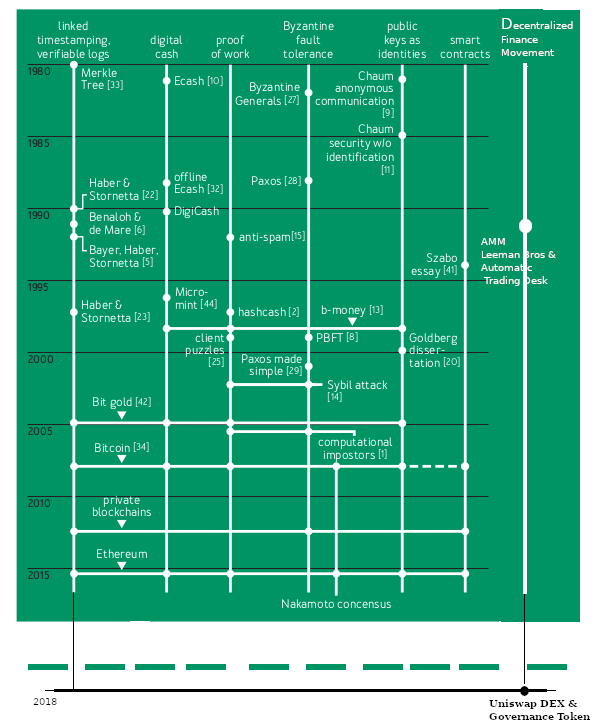
\includegraphics[width=0.38\textwidth]{narayanan3.png}
    \vspace*{-0.3cm}
    \caption{Blockchain key ideas including Nakamoto consensus and DEFI (adapted from Narayaran and Clark, 2019)}
    \label{fig:narayanan}
\end{figure}
 
 The Ancient Greek astronomers had defined the logarithmic magnitude system and introduced concepts of limits and infinitesimals that would become the basis of differential geometry, calculus and numerical methods, readily found today in open source tool-kits or  libraries for the development of astronomy, many of these built by the community; eg Astropy.
 
 It is now known after a plethora of multi-disciplinary studies including that of \citet{Freeth2021}, that during the `decline' of Ancient Greece the first analogue `Computer' was temporally `lost' to most of the technological world, until when in the fourteenth century comparable `advanced' mechanisms were developed and used in Astronomical clock machinery in Europe. 
 
 Now, more than two-thousand years hence, Alan Turin (AT) is widely recognized as the modern 'father' of The Computer for his pioneering  work in the twentieth century that paved the foundations of Artificial Intelligence (AI) and Cryptography. 
 
Cryptography, the basis of OB ledger technology has until now not been much considered for astronomy development or revealed in 'full-text' searches of astronomical peer-reviewed international journal papers, least as a potential interoperability catalyzing agent. In fact cryptography for Astronomy has only been explored as an ancillary technology within data transfer applications like data compression, permission and data fidelity procedures.

Conversely, Artificial Intelligence (AI) techniques like `Machine-learning' and `Data Mining'  have become increasingly relevant for Astronomy in the last few decades as can be measured by the increasing rate of published studies in astronomy and astrophysics peer-reviewed international journals, see Fig \ref{fig:ai}. Some of the studies that depend on AI have estimated the physical parameter space of astronomical sources over the observable parameter space, from large ensembles of data measurements and have led to the classification of astrophysical sources and relations or physical laws that `govern' The Universe. AI technology is proving fundamental in the so-called data-tsunami era of astronomy through these data-science techniques, partly as a necessity of mega-survey's data optimization that depend on: Velocity, Volume, Veracity, and data Variety; each of these constraints and their combination is sensitive to specific science-cases. Short timescale astrophysics events with a cadence of 1 day or less for example for the study of Kilonova transients require multi-messenger observations that depend on real-time AI alert systems to constrain Kilonova specto-photometric models have revealed only in the last few years that a significant percentage of the Lanthanide Universal abundance budget occur from rapid neutron capture, or r-process nucleosynthesis reactions of neutron-rich material in 
 ejecta caused by the collision of two neutron stars, see \cite{artola2020}. Most of the coordinated procedures required for these studies have made direct use of community built software packages including Open Source library packages in Python as well as protocols developed by the International Virtual Observatory Alliance (IVOA). Many ot the python packages include community developed core packages, for example $\textit{Scipy, Matplotlib, Astropy., etc}$  and include affiliated packages, submitted by users and vetted by community development process. Others, for example protocols and software defined by IVOA have also been developed with much success in other programing languages. It is argued that this evolving ecosystem is proving to be increasingly relevant for the evolution of Astronomy not just because of the ease-of-use of the programming languages like Python but because of the nucleation of the community development model that minimizes redundancies and gravitates to best-practice procedures and selfless collaborative opportunities for which resources can be pooled and systems built, tested, modified and enhanced. The Open Source development paradigm has proven and is likely to continue to be causal for many of the tools in astronomy as is evidenced in Fig \ref{fig:astropy} that shows how Python as a programming language plays an increasingly significant role in data-science in Astronomy when the number of papers is taken as a metric.  Although the Python community model and the IVOA software development model have been considerable successful, by themselves they may fall somewhat short in optimizing AOD through interoperability if a digital gold standard for AOD transactions remains largely undefined, a central tenet of this white-paper.
 \begin{figure}
    \centering
    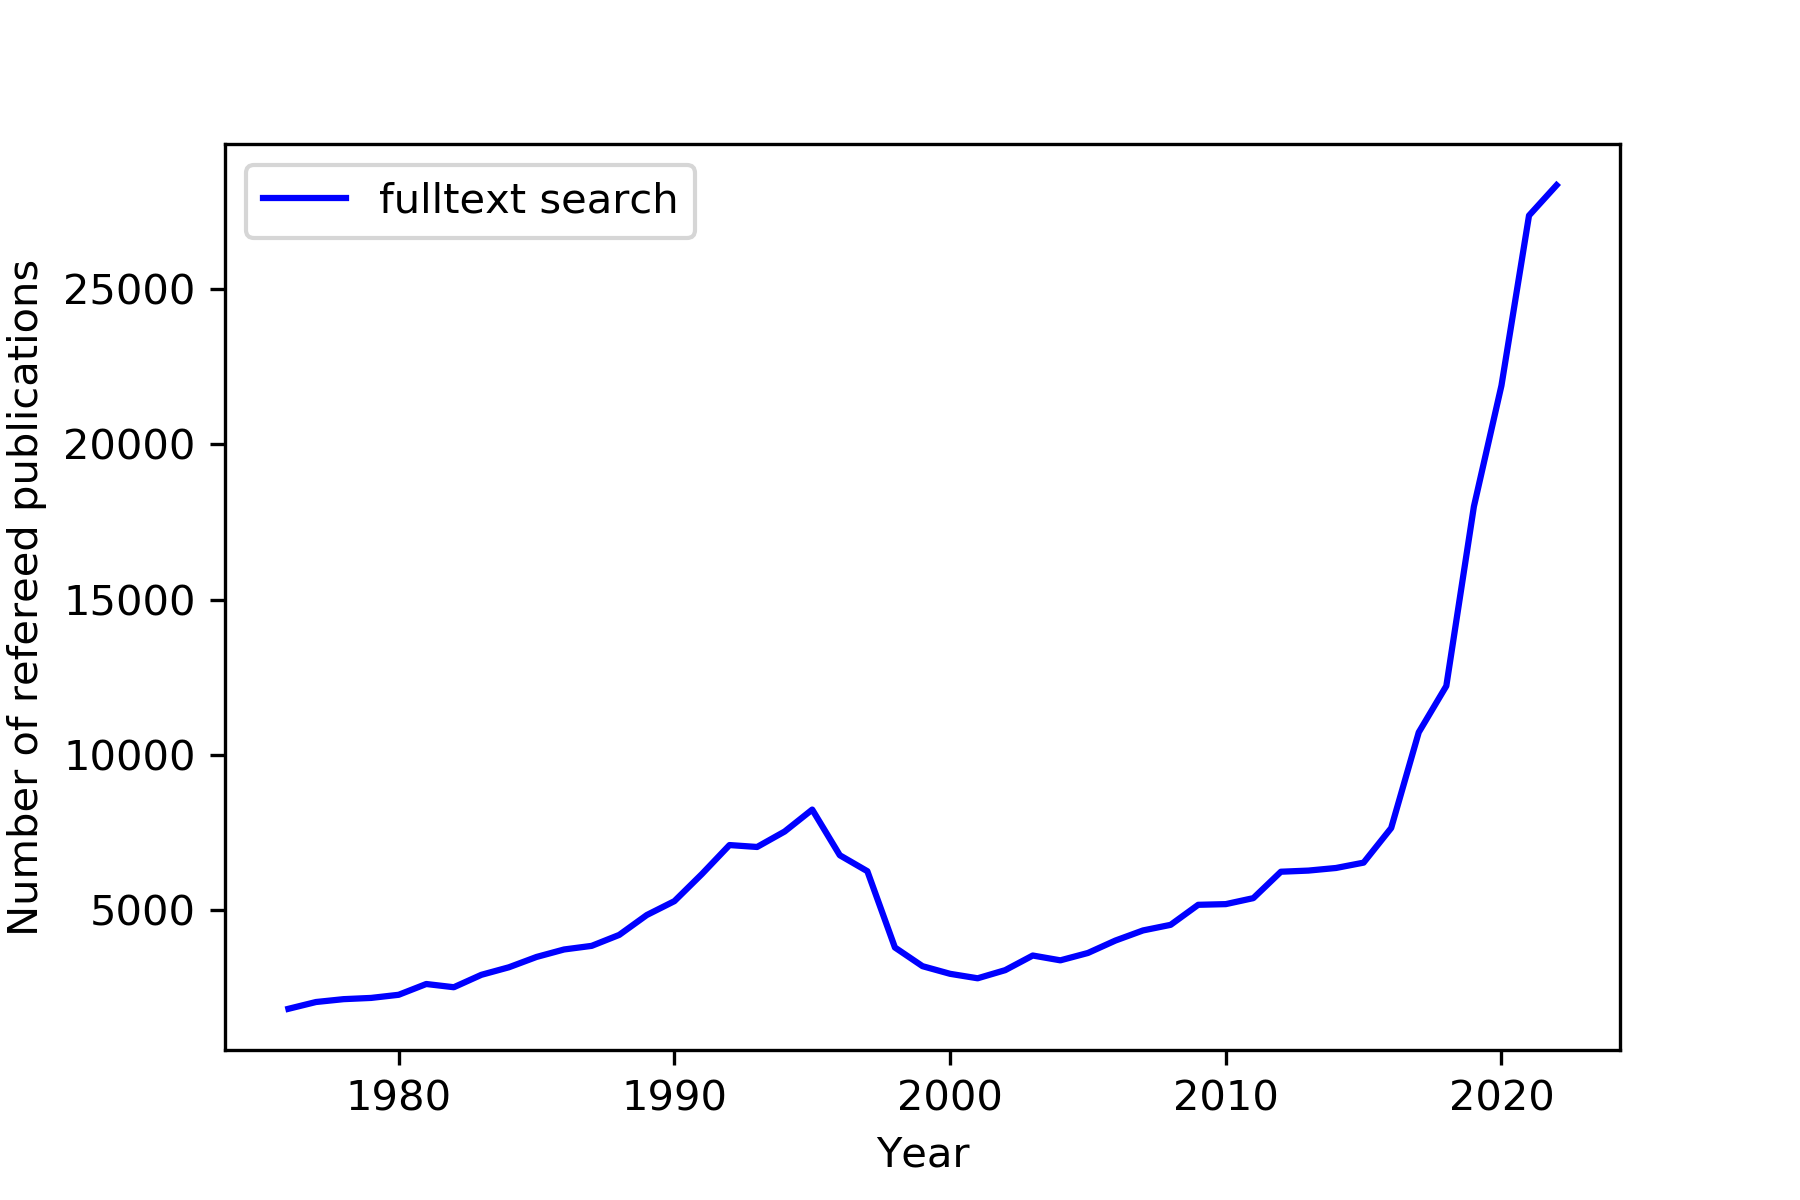
\includegraphics[width=0.48\textwidth]{figs/fulltextai.png}
    \vspace*{-0.4cm}
    \caption{Showing Full-text search for  full:"Artificial" and full:"intelligence" or full: "AI" or full: "machine learning")) AND year:1976-2022) returned query in NASA ADS}
    \label{fig:ai}
\end{figure}

Moreover, the Tsunami data-streams from surveys are not easily accessible for reprocessing by the more broader community, and data-access still depends on propriety periods and to a degree on in-house techniques. An examination of the Vera Rubin pre-processed survey data is now considered. Data from the Vera C. Rubin Observatory, originally: The Legacy Survey of Space and Time once observed is pre-processed and ingested into seven Brokers that have been selected in an Open Community competition call.  This call was made to attempt to guarantee the data bandwidth and ingestion rate of the survey for seven 'Community Brokers' as later selected: Alerce, Ampel, Antares, Babamul, Fink, Lasair, Pitt-Google. These teams contain some degree of centralization since some are more weighted on specific science objectives and skill-sets that rely on a code base and procedures that are not necessarily optimal and community driven across all possible science cases. OB could be used to fund a dedicated Astropy and IVOA community Broker where incentives could be rewarded to contributors via OB Oracles. An example selected to illustrate this point is from experience of the Vista Variables in the Via Lactea VVV survey. After the commissioning, an issue was found in the Cambridge Astronomical Survey Unit preprocessing algorithm by Victoria Santucho (VS) who was completing her licentiate thesis at the National University of Cordoba, Argentina. As part of the science team VS had 18 month proprietary access to the preprocessed data and VS determined in 2012 that the CASU 1.1 pawprint catalogs had systematic magnitude differences due to a 'grouting error' in the preprocessed data (Mike Irwin, priv comm), see Fig. \ref{fig:mapa_dif_Kvsa_Kcasu_grid80_1} when compared to the Vista Science Achieve Catalogues. The effect was fixed in later CASU data releases and resolved internally to the collaboration. Most people outside of the proprietary team who base their studies on corrected magnitudes from pre-processed VVV or VVVx data are not familiar with VS work because by itself this task was not published in any peer reviewed journal. Decentralized Science funding or DESCI via existing governance structures like IVOA \& IAU could be used to address some of these subtleties of open development, mitigate some issues and lead to more open Astronomy development standards that through Federated learning models and appropriate incentive mechanisms based on OB protocols may add guard-rails to increase the efficiency of the  ELT (extract, load, transform) processes required.

\subsection{ The Brokers in the Rubin Survey }

The 7 community brokers as mentioned above are  themselves responsible for source-matching \citep{bellm19}. The FAIR principles for open astronomy science as reported in \cite{2022arXiv220310710O} and \cite{molinaro21} have proven useful for IVOA software development. However across the wider community various groups often adopt different reduction and analysis methods and techniques for particular problems, for example: different source cross matching algorithms have been developed that offer clear advantages and biases on sample selection that are sensitive to source-type, colour, whether the sample is magnitude or volume limited, etc,  within  different bandpass filter sets.
 Could the data-streams use OB protocols to protect data provenience uniting analysis strength across brokers over different wavelengths, AI learning methods, and data models through different community institutions and organizations? In this whitepaper OB is proposed as this missing link in an environment where the half-life function of US PhD majors in astronomy is in steep decline and where projects are becoming much more reliant on team science and access to new technology developments especially in developing countries becomes increasingly difficult since the burden of the opportunity cost to technological development or innovation is denominated in USD and in some cases where inflation and public and private dollar denominated debt is at an all time high, these technological developments are often near prohibitive.

\emph{Our goal then is to discuss the Bitcoin OB Nakamoto standard, and to identify useful elements for a potential base-layer stack for the Open Development of Astronomy including the on-boarding of existing astronomical organizations and institutions.}

\begin{figure}
    \centering
    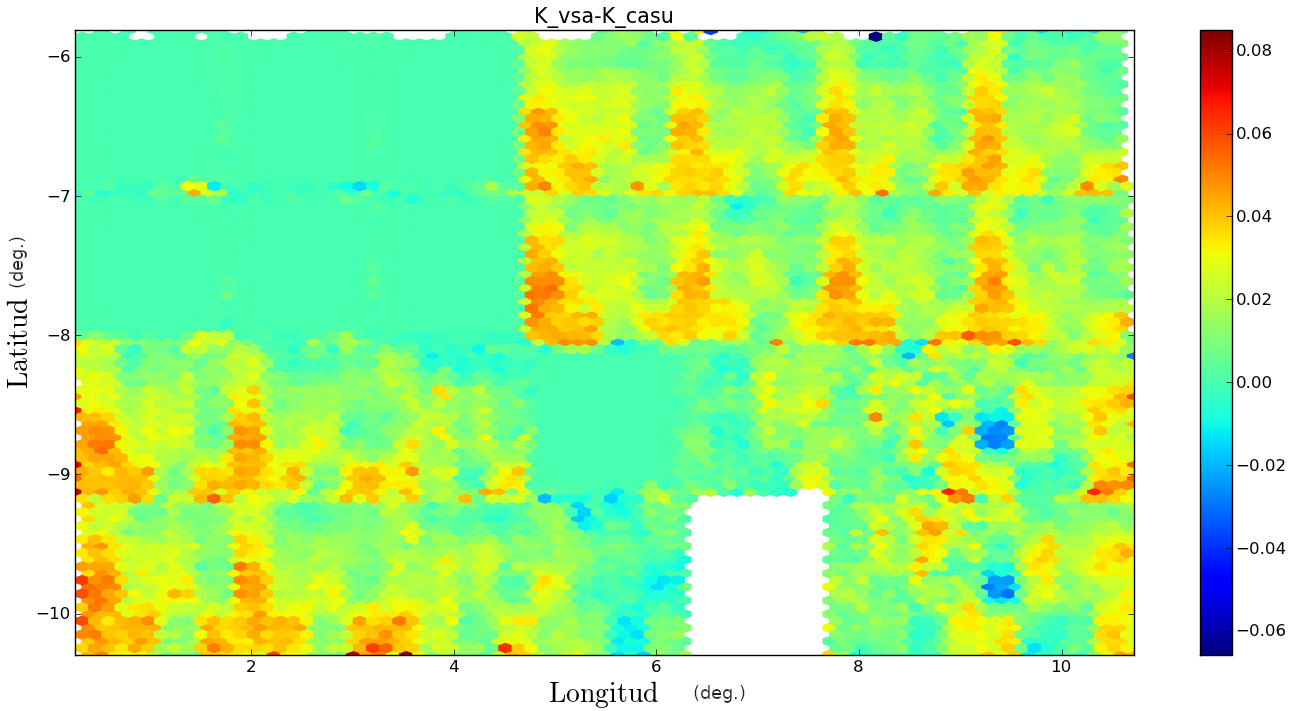
\includegraphics[width=0.38\textwidth]{figs/mapa_dif_Kvsa_Kcasu_grid80_1}
    \vspace*{-0.2cm}
    \caption{Binned Ks magnitude differences (in mags) between Vista Science Achieve and Cambridge Astronomical Survey Unit Catalogue data, caused by a grouting error in preprocessing, found during the VVV proprietary period of 18-month by Vicky Santucho and confirmed by Mike Irwin (priv communication)}
    \label{fig:mapa_dif_Kvsa_Kcasu_grid80_1}
\end{figure}


\begin{figure}
    \centering
    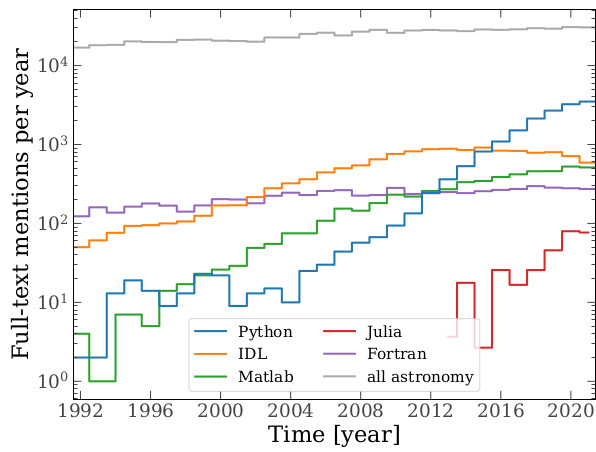
\includegraphics[width=0.38\textwidth]{figs/2206.14220.jpg}
    \vspace*{-0.3cm}
    \caption{Reproduced from Astropy Core paper showing Full-text search for 'programming language' returned query in NASA ADS}
    \label{fig:astropy}
\end{figure}

\section{Open Blockchain as a corner-stone for Astronomy Open Development?}
\label{sec:bc_review}

As emphasized in the previous section and in Fig \ref{fig:narayanan}
, DEFI and DESCI are much rooted in OB protocols including the Nakamoto consensus. Initially, any AOD DESCI OB network will likely depend directly on DEFI protocols for seed funding to permit capital in-flows from more general DEFI liquidity markets as determined by DESCI community governance so these two key-ideas may be notionally considered as separate. AOD liquidity might also flow into more general DEFI liquidity markets (through staking, yield farming, loans, prediction markets, etc), since projects require multi-year planning, costing and OB stable coins may also be used to mitigate against inflation. All decisions must be strictly determined by effective governance on a case-by-case basis that could be done off-chain through a 'snapshot' \footnote{SNAPSHOT: https://docs.snapshot.org/} governance voting poll or via L2 OB. Nevertheless success or failure of AOD tied to OB through the Nakamoto consensus will ultimately and more adequately be determined by the wide-spread use of community developed applications and carefully defined metrics by the community. \cite{arvindandclark2017} make the salient point that the main challenge for wide-spread adoption of decentralized OB ledger technology lies in its utilization by existing users (and institutions) and not in new users from new blockchain institutions. Considering that modern Astronomy has been driven by hardware and software (eg: CCDs, Python, Astropy etc) developments then it may be somewhat surprising to note that unlike AI, OB as a technology has heretherto not been much considered in the Astronomical literature even though funds for instrumentation development are scant, an obvious motivator for this WP. Nevertheless bitcoin has been the commodity and index with the highest ROI on timescales of three years or greater. A model heuristic of this WP centres on highlighting this discrepancy and proposing solutions in the context of the data Tsunami Era, one in which collaborative mega-projects require use of so-called Public Astronomy Brokers as open as possible to community development and when the necessity of technological cooperation is paramount.  

It is further noted that the conservation of the M2 money supply is not time-invariant like are other fundamental physical constants in The Universe since it depends on central bank issuance through highly centralized financial institutions like the US Treasury and Federal Reserve and foreign policy that directly affects other so-called sovereign institutions in other Nation States that have dolar denominated debts. In fact this affects most other levels of government that are often inter-dependant. Sound money on the other hand as a concept is rooted within principles of Austrian Economics  \citet{Hansen2020Book} and although somewhat beyond the scope of this paper has set some fundamental constraints on OB ledger technology. 
DEFI and DESCI are self-consistent ideas that depend on smart-contract automatic market making technology (AMM) to facilitate token swaps and more complex transactions without third party intervention (eg: NFT royalty paying transactions) via DAPPs through (1) Decentralized Exchanges (DEXs) like (2) `UNISWAP' etc. UNISWAP is chosen fiducially because it was the first DEX to offer a massive governance `airdrop' that to-date maintains a large fraction of the locked Total Value (TVL) of all DEFI protocols, except bitcoin and perhaps ETH \footnote{\href{https://defillama.com/protocols/dexes}{DEFI LAMA}}. Although the Uni and ETH tokens were pre-mined and have been funded by Venture Capital and Angel investors no doubt with a degree of centralization, some balance must be sought and reached so more centralized protocols should not necessarily precluded a-priori from taking part in AOD. The Uniswap Dex maintains about 4 billion USD in TVL could be argued to be a valid DEFI protocol that sets-out to overcome the pitfalls of centralized banking and financing in different industries including centralized fractional reserve banking, a central tenet of the Nakamoto Protocol as referenced in Bitcoin's genesis block \textrm{coin-base field} \href{https://www.Blockchain.com/btc/tx/4a5e1e4baab89f3a32518a88c31bc87f618f76673e2cc77ab2127b7afdeda33b}{HEX to ASCII}:  'The Times 03/Jan/2009 Chancellor on brink of second bailout for banks' \footnote{\href{https://hackernoon.com/chancellor-on-brink-of-second-bailout-for-banks-where-to-find-this-on-the-bitcoin-blockchain-hm4k34v4}{Hackernoon article}}, and in a plethora of emails (and reply's) by Satoshi in the cypherpunk's mailing list, that relates energy and time or Power to technology for all transactional based system as examined more thoroughly in the following subsection and in Sec. \ref{sec:energy}.

\subsection{Selected blockchain primitives, key-Ideas and other background knowledge for AOD}
\label{subsec: review}

\cite{arvindandclark2017} show insurmountable evidence as do other authors therein that standard OB protocols are much rooted in academic studies of cryptography. Fig \ref{fig:narayanan} is an adaptation of fig1 of \citet{arvindandclark2017} with the addition of a key-idea or related notion: The Decentralized Finance Movement or "DEFI" that through a `non-custodial' or decentralized exchange "DEX" may issue governance tokens to fund open development incentive efforts. There is much evidence that DEFI was already implicit in the Nakamoto consensus from the outset. As a notion it is referenced in the white-paper as in the `cryptographyat metzdowd.com' mailing list emails from Satoshi in October and November 2008, and in the bitcoin genesis block as mentioned earlier. In the same spirit a DEX enables automatic market making (AMM) token swaps that also provides incentive fees for liquidity providers that depends on smart contracts first proposed by Nick Szabo as an important Blockchain primitive in Extropy \#16 \footnote{\href{ https://archive.org/details/extropy-16}{Extropy \#16}}. The term `smart-contracts' is unrelated to AI but more related to the concept of automatic P2P transactional conditioning, through cryptographic signing that does not technically require human intervention. Alice and Bob can be machine and machine!  In any-case, a `smart-contract' can be automatically executed on the `cloud' via a `trustless' financial rail system like the Bitcoin network. The transaction (Tx) contracts via 'non-custodial' community built infrastructure will automatically be executed prohibiting at the protocol level interference from any third party. Initially developed to omit the need of a centralized order book, a DEX should minimize other counter party risks to contract execution, for example web Framework server failure, like that suffered by INFURA Denial-of-Service (DOS) attack to its price Oracle which unpegged US stable coin values that incurred million dollar losses in Dec 2019 to the Compound protocol, so caution and much care of infrastructure selection and implementation must also be had and periodically reviewed by the Astronomy community. In fact INFURA itself is subject to US regulatory conditioning, that also represents a potential attack vector for true open development since addresses can be blacklisted, including whole countries or regions via metadata filtering by government agencies and the like. This was experienced in Jan 2023 when in a test SG tried to access UNISWAP from Cuba without a VPN. So, a more transparent WEB5 framework may be required for our specfic needs. Following Szabo's definition, \href{https://www.fon.hum.uva.nl/rob/Courses/InformationInSpeech/CDROM/Literature/LOTwinterschool2006/szabo.best.vwh.net/smart.contracts.html}{Smart Contracts} could integrate into base-layer applications like Oracles to automatically in-jest data from third-party data-feeds like NASA ADS publication metrics within a research subject, field, key area,  or even institution. All counter party risks must be averted in contract-design if true decentralization is to be met. Governance through voting must also be thoughtfully contemplated and implemented here. Note:  More details on the notion of a DEX can be found in \cite{uniswap2019_angeris} who explore technical details of UNISWAP and its use as a financial DEFI source.

 \begin{figure}[ht!]
  \centering
  \caption{Historic Price (USD) function of BTC in time (Years), as a potential underlying store-of-value for Astronomy Open Development (AOD). The figure shows the fair value (middle green), and bubble peak (red lines) fits as modelled by Cowen et. al; (2023) for 3 prior market-cycles that are dependent on the bitcoin block reward halvings every 210,000 blocks and the following (estimated) halving as white and red vertical lines, respectively.}
  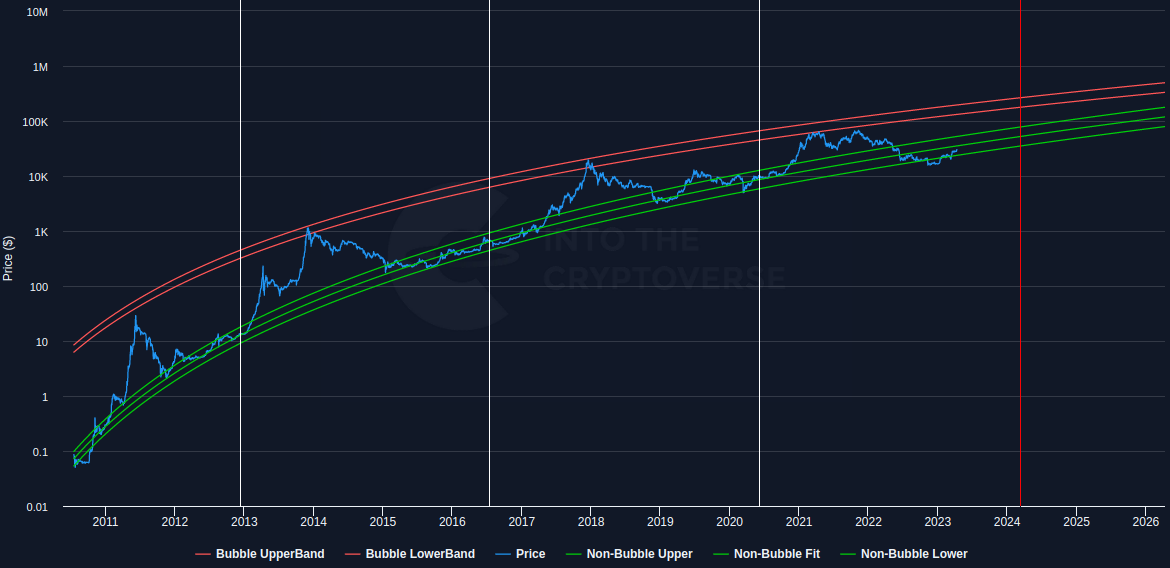
\includegraphics[width=0.4\textwidth]{figs/cowen3.png}
  \label{fig:cowen}
  \end{figure}

\begin{figure}[h!]
    \centering
  \caption{Historic global Crisis, Figure taken from \href{https://en.wikipedia.org/wiki/Global_recession}{wikipedia-commons} adapted from data Reinhart and Rogoff (2009) depicts the binned instances of global crisis (Y-axis) for individual countries that grew in number exponentially before and after the US Nixon administration pulled out of the Breton Woods accord unilaterally that required physical gold backing to USD money printing.}
  \label{fig:crisis}
  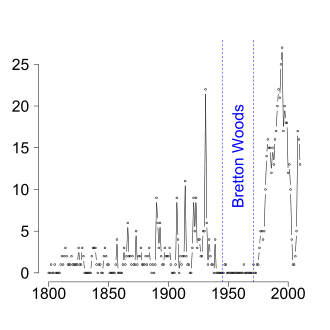
\includegraphics[width=0.5\textwidth]{figs/330px-BankingCrises.svg.png}
\end{figure}

\begin{figure}[h!]
    \centering
  \caption{Figure taken from \cite{milo_2018} depicts the falling half-life rate in Astronomy and Astrophysics and other STEM fields}
  \label{fig:F4.large}
  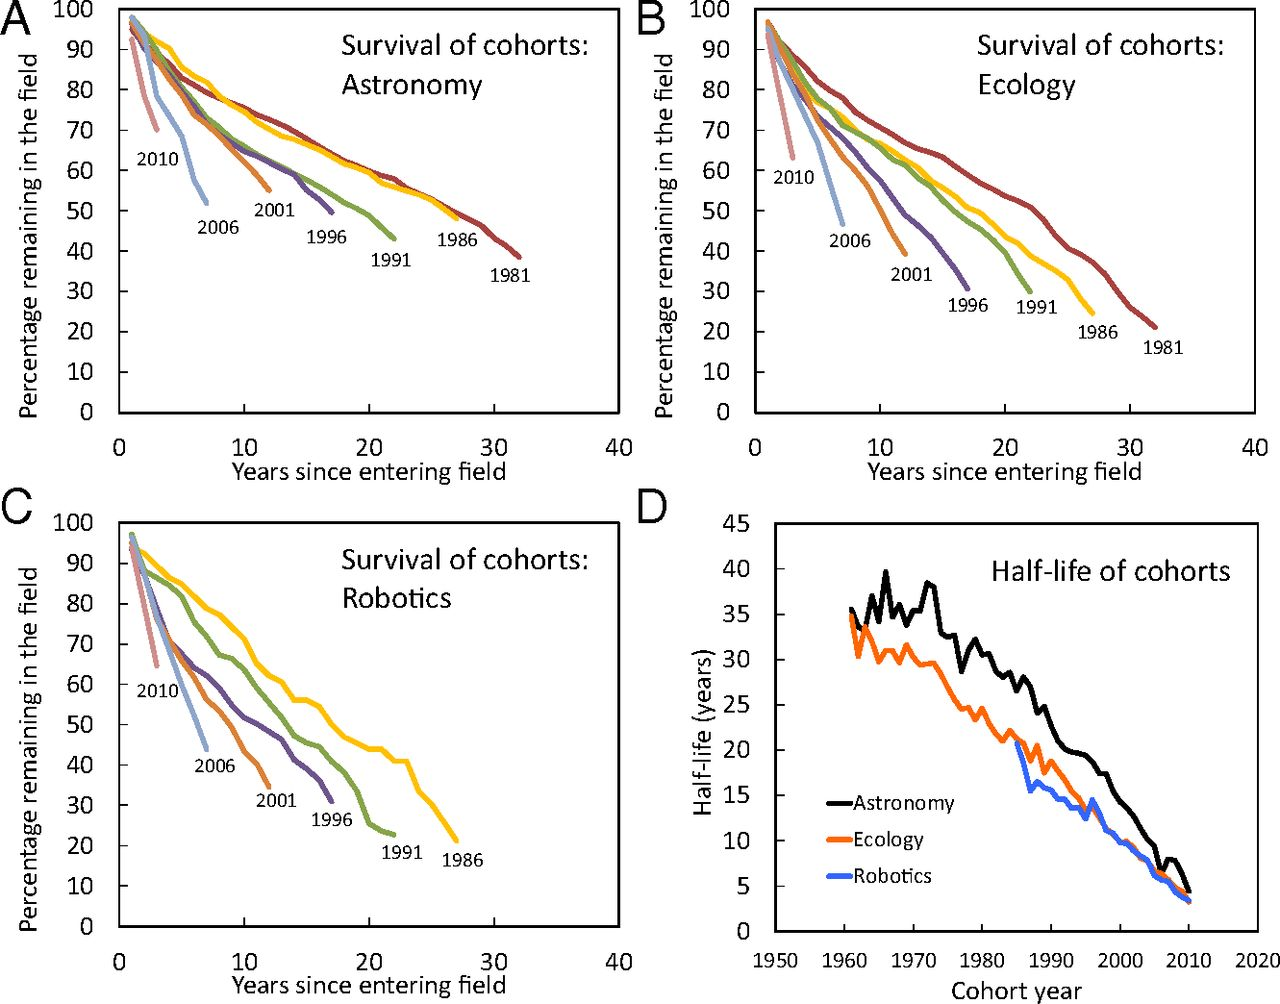
\includegraphics[width=0.5\textwidth]{figs/F4.large.jpg}
\end{figure}
This WP assumes the Nakamoto OB Consensus from the white-paper of \cite{nak2009}, subsequent Bitcoin Improvement Proposals (BIPs) and subsequent selected open-source synergies from other chains that may form a base layer store-of-value for AOD so it should be said is somewhat blockchain agnostic. Although the Nakamoto WP was first published in Cryptography mailing list, the very ideas contained therein were discussed in CPunks, during the 90s; by leading academics. Suffice to say, Bitcoin is the first global financial anonymous network with the following key properties: its proof-of-work consensus algorithm makes it highly secure: resilient to brute-force attacks, it is the only crypto asset that is considered a commodity by US regulatory institutions like the SEC, CFTC and OFAC, and not an unclassified security in an unregulated centralized exchange. It has remained since its inception the crypto asset with the largest market-cap, bar none and forms the base store-of-value of all the crypto assets. It includes a block-size constraint that allows full-nodes to be run even on a Raspberry Pi currently with a couple of TB of disk space. Its supply function is capped at $21\,000\,0000$, and new blocks dependent on miner rewards with a two-week difficulty adjustment. It can be updated, via bitcoin improvement proposals (BIPs). The POW consensus algorithm gives it the security that is correlated with chip development technology, now via ASICs. It has proved to be a valid store-of-value with an ROI superior to other global commodities and indices eg: USD, Gold, S\&P 500 on times-scales of several years and although on shorter time-scales (less than a ~ year) the bitcoin price (in USD) is  volatile, on-chain analysis indicates that over time volatility is decreasing. However the BTC/USD is still somewhat correlated to global financial markets however on longer time-scales bitcoin volatility as measured in USD is falling \citep{wang2022} which might be somewhat expected until it reaches monetization status, something estimated to occur over the next two Bitcoin cycles (approximately 1 decade in time) given current trends and extrapolation of the fair value function in Fig \ref{fig:cowen},  when the bitcoin total market cap is expected to surpass that of gold. 

The latest BIP341 major update occurred at the end of 2021 has added scalability to Bitcoin's network since it allows for complex scripting in the witness portion of the transaction which is where the signing portion of the metadata is also contained. The earlier Lightning BIP was built on-top of Segwit and provides smart-contract capability for AOD applications via Ordinal Inscriptions of Layer 1 that runs on-top of a Bitcoin Core full node. Ord is an opensource software released by \href{https://github.com/casey/ord}{Casey Rodarmor} between 2021-2022, who was not a Bitcoin core dev during that time, attesting the power of open source community development. As Casey has said it was inspired by Satoshi Nakamoto's idea of the indivisible satoshi as an `atomic unit' for Bitcoin in what Casey has subsequently coined `ordinal theory'. Each satoshi has an ordinal number that depends on when the block was minted giving a maximum of 2.1E15 inscriptions. Discussion on the basis of \href{https://bitcointalk.org/index.php?topic=117224.0}{Ordinal theory} began over a decade ago. In fact no BIP was required for ordinal inscriptions. Other bitcoin usage that inserts arbitary data to the Bitcoin blockchain with BIP also exist like \href{https://dev.rootstock.io/rsk/}{RootStock} sidechain merge mining which has also been designed as a smart contract platform for bitcoin. Nevertheless other perhaps less secure `open' Blockchain protocols as previously mentioned may offer some temporary advantages and many issues must be considered including liquidity seed funding and functionality including scalability, Tx costs, Market cap, ease of use, developer numbers, technology standards, cross chain metric analysis as well as other indicators for other L1 chains. This includes Ethereum, DOT, and other chains. Some of these alt chains have helped in the technology development of Bitcoin network notionally as testnets. The Litecoin group of core-developers for example have helped develop and test the lightning network. Many alt L1 have thriving developer communities, DApps and billions of USD in locked liquidity and are part of the burgeoning Decentralized Finance Movement whose protocols offer some advantages for AOD and seed-funding possbilities from DEFI grant funds, that may all help seed AOD. Most interestingly Bitcoin unlike other pre-mined Blockchains like Ethereum and other tokens are not as much affected by more centralized liquidity markets in which venture capital or angel investor funds may dictate or even stymie development. 

Sec. \ref{sec:use-case} is an attempt at an institutional map of the Astronomical Observatory of Cordoba/IATE. Blockchain dynamics are considered for its various sub-units departments, research groups, programs, educational, academic etc., functioning including "Telescopio Itinerante", "Noche de los Museos", "Museum del Observatorio Astronomico", "Library", "FOF workshop", "Olympiadas de Astronomia", etc as identified. The IATE-OAC has over 80 staff including permanent academic staff, graduate and undergraduate students,  CPA (Technical and auxiliary staff) all which make up an otherwise thriving ecosystem. It is argued that for successful open protocols in Astronomy, an incentive system must work for these existing units of research, educational and out-rearch, so there is a necessity of liquidity partitioning to direct to Open Development despite funding challenges that are rooted in challenges of the existing system of funding and financing.

%Smart contract first coined by Nick Szabo have nothing to do with AI but instead related to the concept of automatic conditional P2P transactions that obviate requirement of a third party that may more often than not be a centralized entity. Smart contracts may be  automatically executed by one or several parties. According to a \href{https://www.fon.hum.uva.nl/rob/Courses/InformationInSpeech/CDROM/Literature/LOTwinterschool2006/szabo.best.vwh.net/smart_contracts_2.html}{community vetted smart contract protocols} are useful data-stuctures for open Blockchain development that have applications including Oracles that could involve tokens and nodes that validate transaction and receive data from external data feeds. These could be useful to adjudicated resources using community established metrics that may include publication rate in international refereed peer-reviewed journals or as  a research subject or field, group or institution, including macro metrics like GDP increase towards science and development could be taken as  valid metrics. 

Governance protocols based on smart-contracts are identified as part of potentially successful AOD infrastructure, since the voice of the community may be efficiently enacted via census voting etc; Prediction market protocols could also be used to help AOD mitigate against stochastic ill-effects that may cause restrictions to Open development caused by other status-quo 'hard-wired" funding mechanisms. For example in Sec. \ref{sec:btc4} we examine the TFlop computational issue facing Argentine Astronomers (mostly N-body, and Grid), in which HPC Argentine Research Scientist are at a disadvantage since TFlop capability is disproportionately expensive as is most new technology, priced in USD. So delays of years to obtain project money to start building HPC infrastructure puts Argentine Astronomers on an uneven playing-field. In fact, it was stated in the Jornadas de Computation de Astronomia de Argentina (Nov 2021)  in which the IATE organizers invited members across all the astronomical institutions in Argentina to discuss these issues in a workshop, that: pooling resources is necessary but not sufficient because of rising capital costs to UPS, air-conditioning, rising energy costs, network core infrastructure costs etc, so research projects often have to be scaled back in response of these elevated costs or depend on external  collaborations and infrastructure. In Fig \ref{fig:crisis} we reproduce the historic global crisis function of nation states that depicts an exponential increase in crisis instances during periods when `sound money' was  difficult to come by for many national governments of the world. It is concurrently noted that these periods affect and retard astronomy open development since more essential funding priorities dominate that force governments to use all available funds to cover the bare essential necessities. We emphasize from this figure that during the Bretton Woods accords, or the period within the de-marked broken blue lines that the occurrence of financial crisis takes a value near a global minimum. 

Could the Nakamoto consensus as the go-to store of value or sound money base protocol and subsequent BIPs usher-in a new period of stability and even innovation for AOD? 

In Fig \ref{fig:F4.large} we reproduce the empirical half-life function for astronomy and astrophysics PhD majors as well as other STEM fields within the US Public University System. It is clear that this figure shows an exponential rate of decline.  In this section we have discussed the current and historical situation that has underpinned the negative effects of Astronomy development with examples. Some Blockchain primitives and protocols are identified, selected to complement Open Astronomy Development.  In Sec. \ref{sec:btc4} a simple idea of implementation and on-boarding for our model of Astronomy education/development and research via open development is proposed via Astropy, the leading Open Developer community tool-kit by Astronomers for astronomers and the International Virtual Obseratory Alliance (IVOA), where software interoperability standards have been defined to-date with much success. In Sec. \ref{sec:btc5} conclusions drawn and some discussion on a possible future course of action plus an NFT collection case-study to celebrate 150 years of the Observat\'orio Astron\'omico de Cordoba, the former National Argentine Observatory. 

\subsection{Early Blockchain Fundamentals}
\label{subsec:fundamentals}

The Turing complete programming languages like ETH (\href{https://github.com/ethereumbook/ethereumbook#readme}{Mastering Ethereum}) have loops and are able to iterate infinitely and have central actors (Founder, Cofounder, VC-funds, etc). Bitcoin on the other hand is Turing incomplete, purposely built to be much simpler, it has proven over a decade (see Fig \ref{fig:cowen}) to be a excellent store of value when compared to the USD over time-scale of a few years. Advanced Smart Contracts capabilities were never part of the immediate scope of the original implementation. Whereas Bitcoin was primarily designed to be a P2P form of electronic cash, other Blockchain like Litecoin were used to test implement the Lightening network and other more complex smart contract capabilities in other layers and side-chains. The Ethereum Blockchain has also shown itself to be a successful Blockchain for more advanced smart contract capabilities, and has been defined by its lead developer to be a “World Computer”. There are many excellent sources in the Literature on this topic, suffice to say that Bitcoin devs with BIP XXX YYY have implemented advanced smart-contract cababilities on layer 2 and that below we will concentrate on atributes of a Token for Astronomy choosing a hybrid approach based on ETH and BTC liquidity in the section below in which we describe aspects of our Astronomy OD model.
 

Preceding BITCOIN, many advances in Blockchain technology were made in works like Chaum (1983), Chaum, Fiat Naor (1989), Rivest and Shamir (1997). Haber and Stornetta in 1994 building from the literature as well as from their own paper in \cite{Haber1991wi} put the first Public OB system into practice in the New York Times newspaper classifies. This being the first accredited ledger that was a digital signature time-stamping validation service named "Surety", fourteen years prior to Bitcoin. 

However the first decade of the 21st century gave rise to arguably the most important Blockchain system, the Bitcoin standard, published anonymously by Satoshi Nakamoto in 2008.  In the first block, see Figure X: Satoshi made reference to the Times of London article that reported that the then U.K. chancellor was considering a second Bail-out round of the largest UK Banks. Satoshi, a likely pseudonym has demonstrated affinity with the academic literature since Satoshi much cites the academic literature. According to some studies may represent the work from mostly one individual (MOOC Blockchain, Princeton), although definitive evidence remains somewhat elusive perhaps more evidence will come to light if the early Wallets of Satoshi that contain many early Bitcoin become active. Moreover the identity of Satoshi or any Blockchain OG is a surface of attack to that network so it is no doubt that Satoshi identity is hidden by design, hopefully never be revealed and those early wallets remain forever dormant. Never-the-less Bitcoin the Blockchain network and bitcoin the asset have grown in value more than any other asset classes, including gold, so it could be argued that so far, in the time-frame of years in it's first decade of existence the Store-of-value proposition appears hold and must be not be ignored.

On shorter time-frames less than $\sim 1$ year bitcoin volatility is significantly higher. No doubt compared to other asset or commodity classes like Gold it is measurably young and hence volatility high since if it is to represent a global commodity reference, its market cap will no doubt be more sensitive to external speculative financial capital markets. 

Bitcoin as a world reserve still appears to be partly correlated to other global financial markets. A recent example is the Covid19 black Thursday pandemic that in March 2020 saw BTC price drop by more than 30\% in only a few hours. This appeared to be triggered by the Black Thursday liquidity crisis that swept the much larger global financial markets and the reactions of central bank governments to it as did the Omicron crash of December 2021. The March 2020 crash coincided with a crash in global equity markets that saw stocks suffer the worse losses since The Great Depression" and iconic corporations were "bailed out", like Hertz after a record number of unemployed, filed for unemployment benefits in the US. After about a fortnight, like many blue-chip stocks, bailed out by the US FED via Repo, corporate bond offers, and share buy-backs the bitcoin price (in USD) recovered almost instantly. Against other asset classes including gold and USD, bitcoin appears to be in the short scales at worst, as volatile. 
 
Bitcoin as a technology to solve several problems faced by earlier digital currencies. Having no single point of failure meant law-suits can not be used to persecute it anonymous creators. This adds to network security by processing Hash functions which is adjusted on a two week basis. Some authors, including Andreas Antonopoulos believe Bitcoin and Ethereum Blockchains have the potential to revolutionize open development in science and technology and with 5G roll-out promise unprecedented levels of growth of over 18 percent per year, not seen since the first industrial revolution Waldon, M.  Fig needtoinsertfigure adapted from Walden et al. shows the world GDP as a function of time. These technologies were born out of academia, the occupy wall-street and anonymous movements as a direct response to the 2008 financial crisis that saw a global slump in the world GDP based on the US sub-prime financial crisis  that included a drop in US GDP by 30 \% sustained over several years.
 
Programmable money is not exclusively relevant to human beings but also to machines as participating actors. Hardware evolution is also tied to open development, as seen in the evolution of specialized hardware architecture for Proof Of Work (POW) HASH Function calculations that is developing Application-Specific Integrated Circuit (ASICS) to mine Bitcoin blocks. It could be argued that these developments have outpaced Moore's law.  Wrights Law suggests that the for every percentage increase in the cumulative distribution function of production in any industry equates to a fixed percentage increase in the efficiency of production. So hardware has evolved from CPU intense through to graphic processing units (GPU) and  Application Specific Integrated Circuit  (ASICS), \cite{10.1371/journal.pone.0052669}. A successful model for Astronomy and Astrophysics Open Development would do well to tie metrics of Open Production into the protocol as well as the appropriate incentive mechanism.       

OB are uncensored so a data protocol standard of best practice through governance could be cross validated from an information criterion perspective that includes Oracle feeds for Open Development.  Oracles that receive feeds are penalized if they predict incorrect probability distributions of events or Facts for Astronomy Development prediction markets. 

\section{Bitcoin and the Kardashev model conundrum}
\label{sec:energy}

We now propose to use Bitcoin to reconcile the \cite{kar64} law with physical reality through a more realistic re-normalized power growth rate model than the 1\% model. We first observe the 1\% model fit fails to reproduce real data and violates the memory conservation property, that may actually be required for any technologically advanced civilization and base all subsequent analysis on data from \cite{owidenergy} of the average total power (in one hour) for each year from 1964 to 2021. The 1 \% model fit is shown in \ref{fig:kardashev1} with the data. The form of the fit is clearly inconsistent with the data and obviously produces unfathomable scatter about the data.

%Bitcoin has been described in early sections and previous works to behave as a unit of account, store-of-value and potential medium of exchange.  
This can be explained because the distribution of a random variable X, say Global Power is \textbf{memoryless} if for all real numbers a and b in its range satisfies:
\begin{equation}
P(X>a +b|X>b)=P(X>a)
\label{eqn:memless}
\end{equation}

Kardashev's 1\% model is a geometric series with a non-negative integer common ratio. It follows the probability distribution of the the type of Eqn. \ref{eqn:memless}. Possessing the memoryless property renders this model anathema to the very phenomea Kardashev intended to model as described by Eqn. \ref{eq:2}, reproduced from the original paper of \cite{kar64}:

\begin{equation}
(1+x)^t \approx e^{tx}
\label{eq:2}
\end{equation}

In Eqn. \ref{eq:2}, taken from \cite{kar64}, Kardashev sets x=0.01 for the 1 \% energy growth model and defines Type 1 civilizations as any civilization that consumes an equivalent amount of power as consumed on The Earth in 1964. Using  this growth rate Kardashev proceeds to calculate that Human civilization would reach Type II or the Power attainment equal to the The Sun's total bolometric luminosity of roughly 3.9 X $10^{26}$ W in roughly 4000 years, see Table 1.  \cite{sagan73} accept the 1\% model but slightly re-define the zero point and obtain a similar conclusion for the Type II and Type III attainment timescale. Type III time-scale would be reached when a civilization via say Dyson spheres are able to muster as much Power as would be emitted by all of the stars of their host galaxy. Interestingly \cite{sagan73} following Kardashev additionally suggest an information metric as a second dimensional parameter to that Kardeshev relation but do not generalize the Kardashev fitting function. \cite{sagan73} use a binary tree data-structure to suggest that all the information of The Earth including the contribution of Greek Philosophy would require roughly 2**16 bits. Interestingly \cite{sagan73} propose a data-structure of a similar form to a Hash tree or Merkle Tree since Hash trees like Bitcoin's are in general Binary trees that preserve critical state information of the system. Table one shows the predicted Energy consumption by advanced civilisation from type I to type III, based on \cite{kar64}. We show the two model fits in Fig. \ref{fig:kardashev3} and superpose horizontal demarcation broken lines to indicate the Kardashev and Sagan type I and type II limits as well as the solar Insolation limit. We note that although we have set the Insolation limit as constant it will also depend somewhat on the Milankovitch (Orbital) cycles guaranteeing a non-constant Kardashev growth rate model! First we take the 1964 data and extrapolate it using the 1\% year growth rate model and calculate when the average total power reaches type II. We then fit the actual data with an OLS fit. We also solve our OLS fit to the type II Power limit as determined by \cite{kar64} and \cite{sagan73}. For our re-scaling and assuming Bitcoinization and the extrapolation of Global Energy usage we assume Bitcoin value-layer to also be locked with Global Energy production. so we take the zero-point or fiducial point of type I to Bitcoins 2009 genesis block and type II to be when the block reward halving and estimate that currently the Earth's Civilization has surpassed a type I civilization. In \cite{sagan73} an alternate information metric is considered one that includes information richness of any civilization. This can be represented in a Binary operations even a Binary Tree which share the Hash tree or Merkel tree structure. Interesting, the Bitcoin Network Ledger which contains transaction information of every single Bitcoin transaction may also be used between non-humans. This may be the sense of "Smart Contracts" by Nick Szabo. The Bitcoin hash-rate as a function of time we take to represent a type of Energy Production metric and simultaneously preserve the Information richness required in our model. We take data complied from the International Energy Agency and BP, from \cite{owidenergy} and plot the total yearly power production available for The Earth. In Fig \ref{fig:kardashev1}, we show actual data since 1964 from \cite{owidenergy}. We show two models, the Kardashev Equation \ref{eq:2} 1\% model, taking the first point of the actual 1964 data and a OLS model to the data. Interesting the second last datum point shows a 3 percent decline in production in 2020 (Due to COVID) and a 5 percent increase in production in 2021 breaking the COVID-19 pandemic year! A slump due to the 2008 sub-prime crisis that gave rise to the Nakamoto consensus is shown. The extrapolated model is closely linear!
\begin{figure}
    \centering
    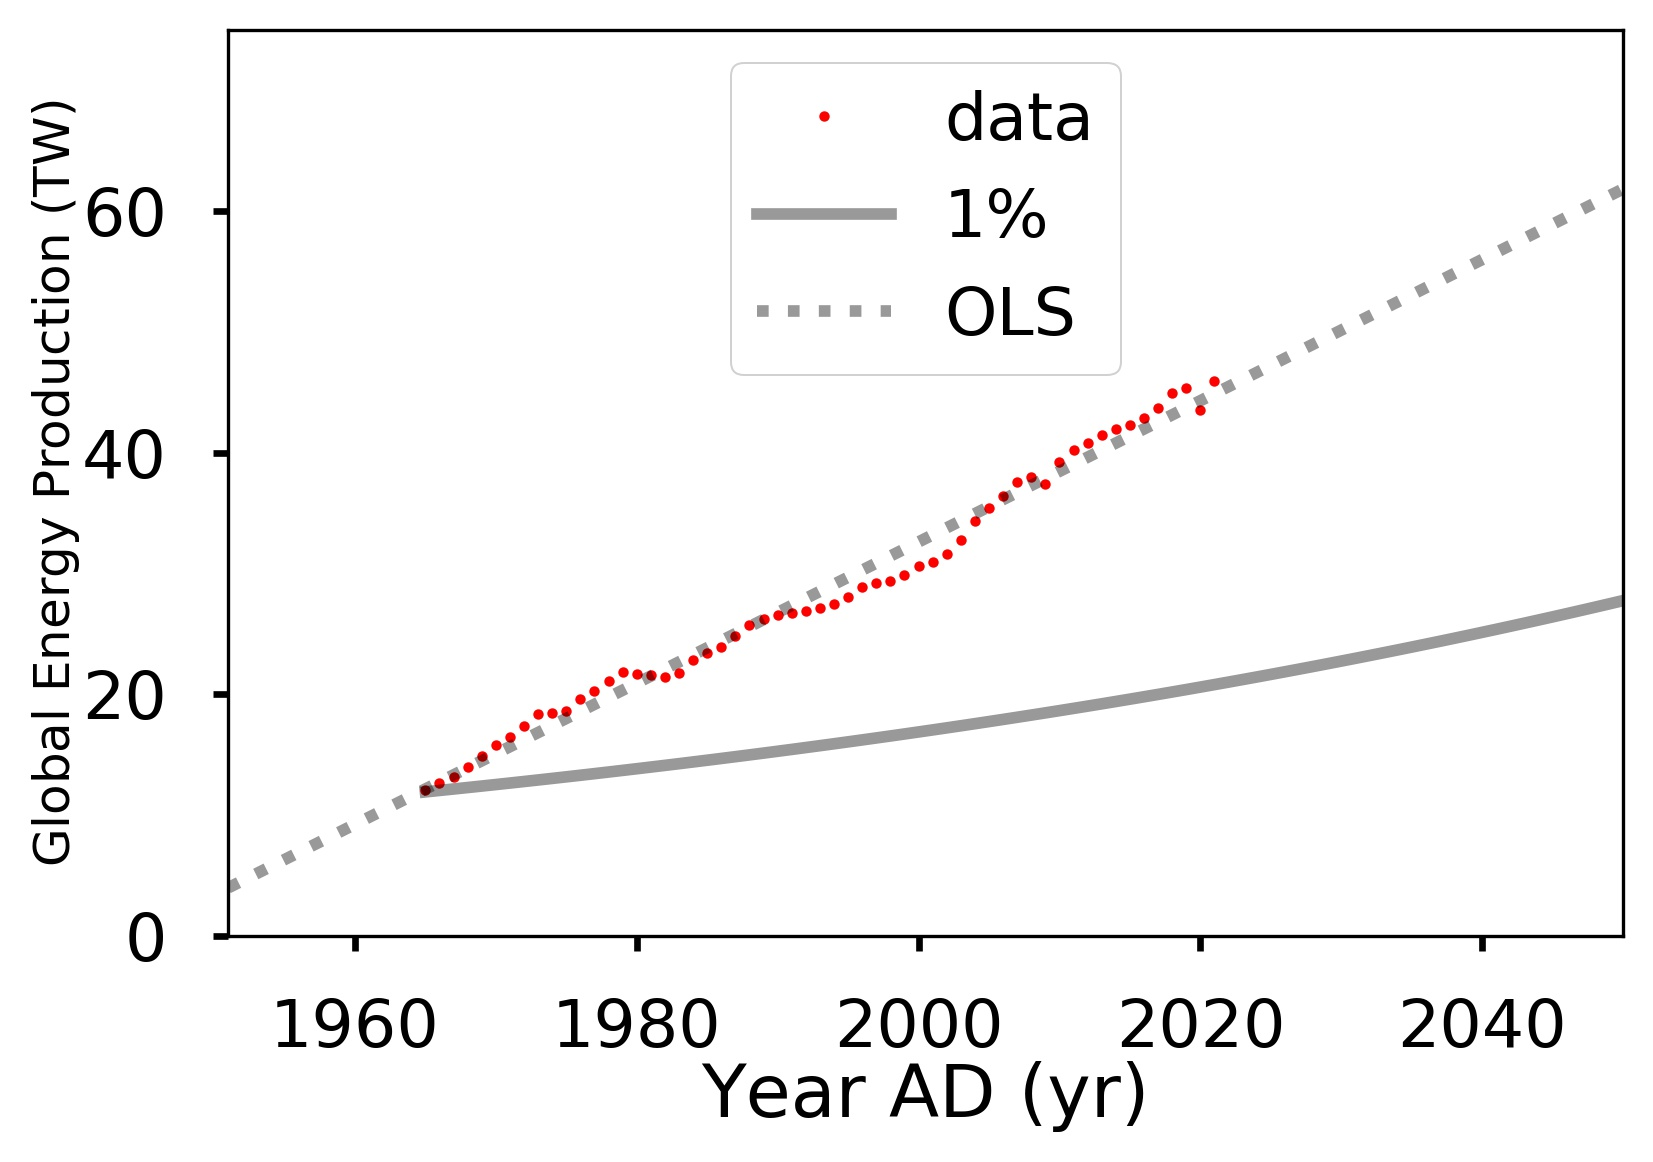
\includegraphics[width=0.5\textwidth]{figs/fig1_kard.jpg}
    \caption{Global average energy production metric in Terra Watts VS Year (lin-lin) from the Owidenergy resource with a Ordinary Least-squares fit and the 1 percent yearly increase model as proposed originally by Kardashev, subsequently by Sagan and later authors. The Scipy Python module was used to do the linear fit.}
    \label{fig:kardashev1}

\end{figure}

In Figure \ref{fig:kardashev3}, we show the same data on a log-log plot and include the Kardashev and Sagan Civilization Types I and II and the Solar Insolation value or the total energy of The Sun abosrbed by the clouds, oceans and Earth's surface. %It can be seen that the original Kardashev limit by \cite{kar64} of 4 TW was already reached but the T1- Sagan limit of 10000 TW from \cite{Sagan73} will be reached in about 20000 years. 


\begin{figure}
    \centering
    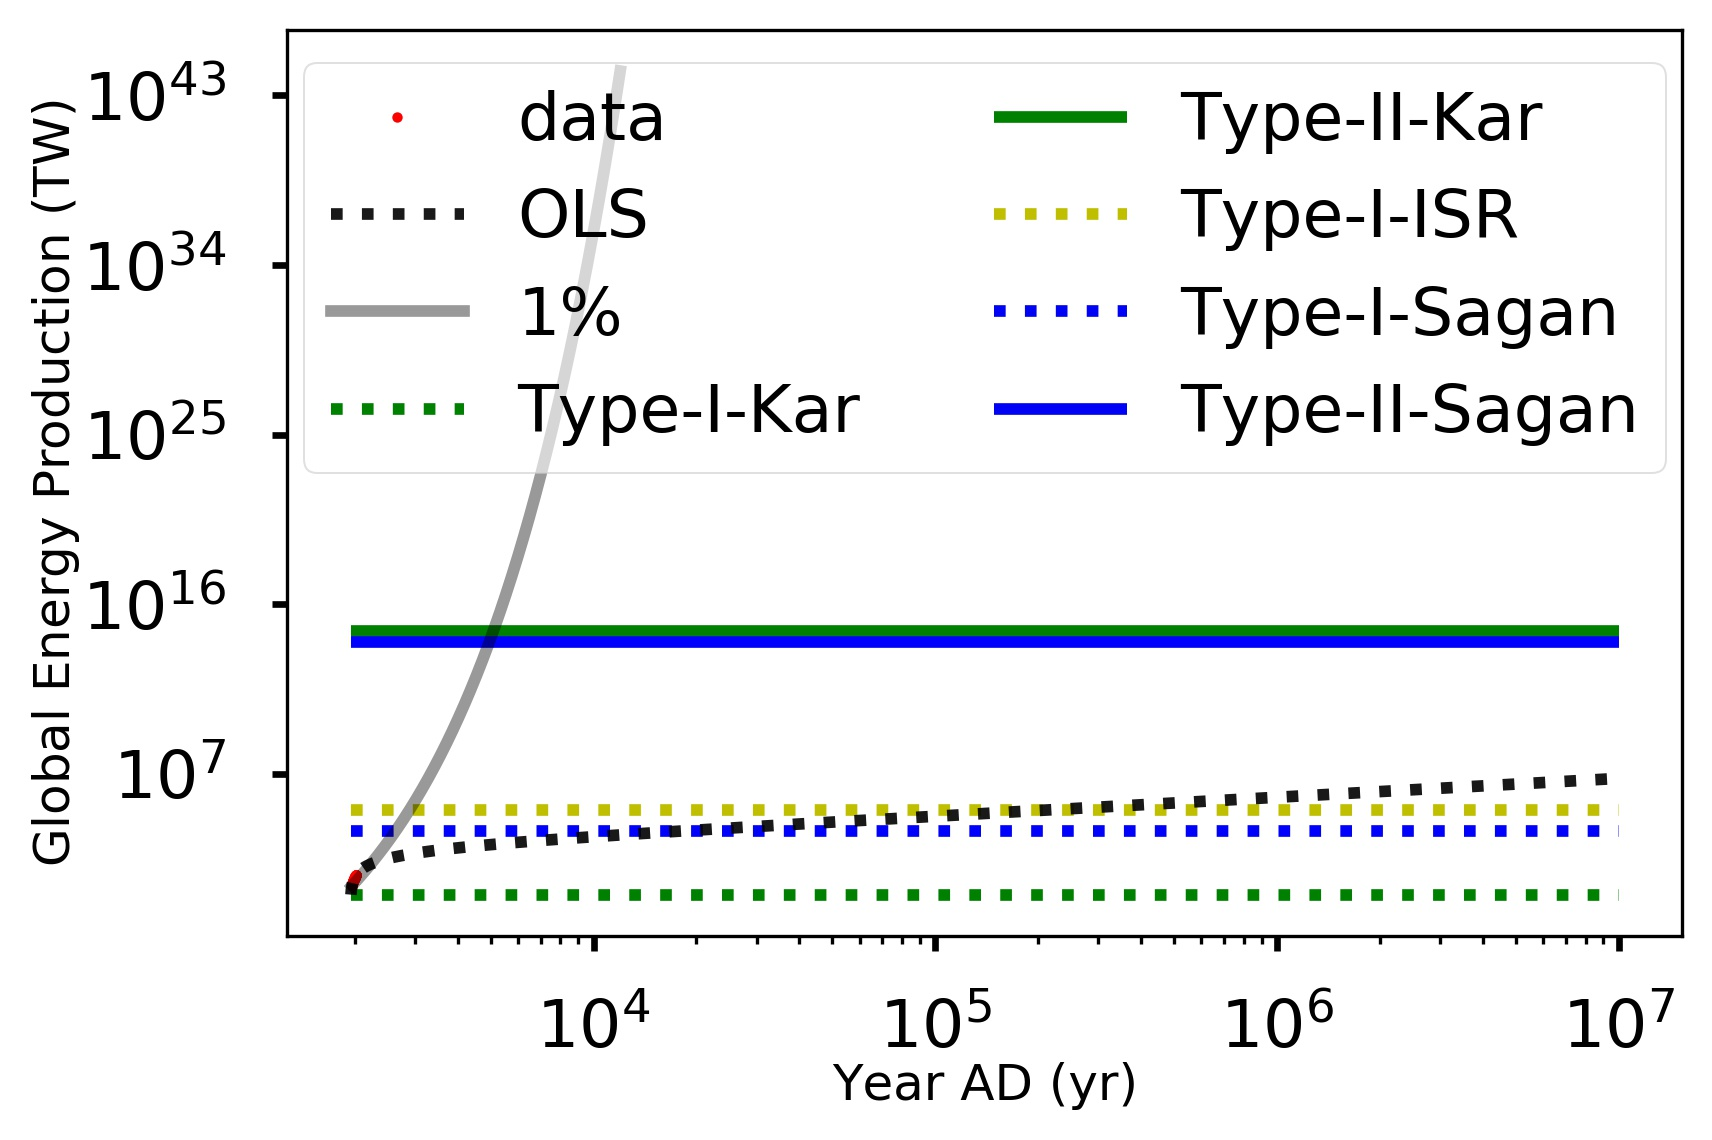
\includegraphics[width=0.5\textwidth]{figs/fig2_kar.jpg}
    \caption{Global energy production metric in Terra Watts VS Year (log-log), taken directly from the Owidenergy resource, with a Ordinary Least-squares fit. The solar Insolation, Kardashev Types I and II limits are shown for Kardashev and Sagan esstimates. The Scipy Python module was used to do the linear fit.}
    \label{fig:kardashev3}

\end{figure}

The figures show that the estimations of time required to reach Type-I and Type-II for Kardashev and Sagan with a simple average incremental extrapolation are indeed significantly off since real world data includes decrements in yearly production as well as yearly increments due to internal and external crisis caused by human-kind. To get a alternate handle on the Kardashev time-scale estimates we choose a Monte-Carlo approach.

First, we take the difference between succesive years of the Energy Production from the Oneworld yearly average data, and randomly redraw from a probability distribution of the data that has a measured Kurtosis of, and a mean and standard deviation of . We do a Skewness test and obtain a test statistic and cv value of, thus we are unable to reject the null-hypothesis and must accept that the Power differences  are consistent with a Normal Distribution. This distribution is then redrawn randomly, and we obtain a mean and scatter of for the years requred to reach type two from different years. Our results show that Type II  time-scales are close to the hubble time.

Considering that on average a new Bitcoin block is mined every 10 min, so 2015 blocks represents nearly a perfect two week interval. This is the difficulty adjustment time-scale that Satoshi chose realizing that the Hash-rate would evolve with time taking into consideration both the effect of new mining technology and variability in mining activity. In actual fact, a bug in Satoshi's Bitcoin Core client code or a zero-error=1 persists such that the the first block of every 2016 blocks is not actually included in the moving average calculation only the last 2015 blocks are considered. This bug can only be changed with a hard-fork that too date is a cost too high to warrant implementation. Now, given the instantaneous hash rate will depend on many variables like seasonal electrical supply costs, technology developments, miner adoption rate, etc., miners may even temporarily switch off mining units. For example, in Southern China in the Summer months the monsoon Wet-Season provides abundant energy supply that drives more intense miner activity such that the total China hash-rate committed may increase by more than 100 \%, with electricity generated from stranded hydro facilities or natural gas flaring that may be otherwise illegally flared (REF). Nevertheless, on the criticism that Bitcoin Network requires as much power as some Countries like Argentina or large cities as New York, confusion is often and unwittingly made between Energy Consumption and Energy Production and comparisons to other the consumption of other industries, often omitted. The Bitcoin energy consumption models by the Cambridge University Judge's University Center for Alternative Finance or simply the Bitcoin Energy Consumption Index puts many of these comparisons into context. The Bitcoin Energy Consumption Index estimates the Energy Consumption by modelling the Bitcoin hash rate with hash computes, using a Normal distribution of basket miner technology (GPU's, ASICS etc), taking into account technological advances in ASICS production, World Energy costs ., etc. Using these model parameters, the CBECI estimate that as percentage of world total energy for Bitcoin will remain below 0.1 \% of the world production over Bitcoin lifetime. Other authors like Antonopoulos argue that the energy cost of the Bitcoin network is near the noise of the total global energy consumption value yet such a cost is a bargain if it leads to a secure a reserve global decentralized and uncensurable financial network. Although Bitcoinization will occur after monitization in this section we start out considering two canonical papers on the subject of Energy consumption for technologically advanced civilizations by Kardashev 1964 and Sagan 1973 and then adjust these models for Bitcoin Hashrate and make a plot in Fig XXX to visualize the evolution of power for Bitcoin over a x year base-line taking the Cambridge Bitcoin Electricity Consumption Index, Bitcoin Use Scale as predicted by: \\

$E_BTC/E_tot < 0.1$
\\

The energy required to operate the Bitcoin Network is within the error budget of the total global energy consumption and although it may be a necessary cost one must take in mind: (i) this cost is to secure the network (ii) that energy consumption is a lower limit on energy production (iii) that a significant percentage of POW hash-rate is powered by renewable energy sources that could if consensual agreement be reached by miners,  holders, governments and the general community, power the Bitcoin Network using renewable and sustainable stranded energy or even within a carbon credit system. Of course on the topic of energy consumption, the \cite{kar64} model or Energy Use function for civilizations is a useful comparison chart to ascertain the current Energy situation of Civilization on The Earth over as long a time baseline as possible to mitigate sensibility of low time-scale variance given the potential of wide-use of Bitcoin adoption as analyzed in this paper.

 \subsection{POW Incentive}

The target hash-rate for Bitcoin is a moving average of the hash rate over the last 2,015 blocks.The hashing power is estimated from the number of blocks being mined in the last 24h and the current block difficulty, given the average time T between mined blocks and a difficulty D, the estimated hash rate per second is given by:\\

$\textrm{H} = 2^{32} \textrm{D} / \textrm{T}$\\

\subsection{Indexing Open Production and Development}
In this subsection the notion of indexing open production metrics is discussed

\section{Open Astronomy development}
\label{sec:btc4}

The Bitcoin network over long time-scales requires an increasing amount of energy for hashing that has been estimated by the Cambridge Bitcoin Electricity Consumption Index as limited to a fixed percentage of the total global energy production. The energy required for Bitcoin's POW consensus algorithm has been criticized for the Power required to operate and secure it. Bitcoin hashing is considered fundamental to the POW protocol for the: (1) production of new blocks, (2) processing of unspent transactions (UTXO). At any time, the hash rate is a measure of the hash-power of the total Bitcoin POW system.  

In this section we discuss use-cases for Blockchain as selected case-studies. Before entertaining this idea we must consider some notions. If we accept that there are bubbles in the bitcoin price volatility and that the btc/USD volatility may be taken as a proxy metric to this volatility then we must examine ways to mitigate against downside volatility for AOD during periods in which the btc/USD is significantly above the average during bubble periods. One metric for this is the 20 week simple and exponential moving average functions or some equivalent which represent periods of fair-valuation. In periods when the daily bitcoin price is well above this band a minimum percentage of total AOD liquidity must be held in stable coins by AOD treasury. Likewise when the btc/USD price is much below the 20-week moving average some minimum liquidity must be held in bitcoin. These limits may be selected as a community via voting to maintain potential value for AOD although some liquidity partitions must be managed more locally depending on the use-case. The following use-cases are now selected across a wide base-line of activities for Astronomy development at the OAC-IATE for (i) funding of a new telescope-system TOROS at an ELT tested site, (ii) 'telescopio itinerante' or itinerant telescope program of the OAC, (iii) re-value historical OAC patrimony, (iv) grant stable coin liquidity pool for granted research projects, that is PICT-PIP, (v) Community Broker for backend of Vera Rubin Survey. (vi) Astronomy software development. (vii) inclusion of mega-project in-kind financing like the CFHT
Letters of Interest to participate in the development of the Maunakea
Spectroscopic Explorer (MSE). 

Of the seven case-types identified, the first four focus on the OAC-IATE ecosystem and the last three on a more global scale so in this context some global salient issues that affect AOD are purported that include so-called global brain drain or haemorrhage afflicting astronomers. In Subsec. \ref{btc2:sec:sub:half} proxy metrics for AOD are proposed that might go someway to restore historic half-life rate function of Astronomy PhD majors in Public US Universities and associated AOD systems as considered. 

With respect to the community broker for the Vera Rubin Survey, it is noted that an expected capacity of 10,000 alerts will be provided every 39 seconds so there is a need for short time-scale and semantically rich science. Triggering Difference Image source, 82 KB per alert means 5 GB per s per full stream. Sixty Second from read-out information needs to get to the Broker system, at least 5 full streams to alert brokers.   For example  Jakob Nordin of AMPEL, requests from the community a standard processing framework for Legacy Very Rubin data, a standard that would enable processing of data-sets irrespective of broker identically and as efficiently as possible, at the moment this is a challenge.  Mathew Graham of Babamul considers that traditional approaches to handle event streams are sub-optimal and sees for back-end work a decentralized network of low-cost components employing commodity AI accelerators and reusable models plus an in-use science data platform for information management that any group can set up on their own at-scale broker for less than 1 USD per day, using Raspberry PI + USB TPUs (4 TOPS), optimal for deep learning models.  Federated Learning for example, which is what Babamul devs have claimed is completely open sourced, could well complement open block chain protocols implementation. Several issues exist within federated learning systems including single-point failure type issues, but also a suitable incentive mechanism to mitigate against data falsification. Blockchain-enabled federated learning can solve these issues as described in \cite{zhu2023} 


\subsection{Half-life function}
\label{btc2:sec:sub:half}

The exponentially falling half-life function for Astronomy majors in US public universities is an alarming metric. It is now about 3 years and has been dropping exponentially since about 1970 or about the same time the US withdrew unilaterally from the International Bretton-Woods accords that tied the 'price of one USD' to an allocation of gold. The desertion PhD function could be considered a global hemorrhage of 'grey matter' or capital flight away from astronomy open development.

\emph{In an open development model scientific contributions from the community should be guaranteed, valued and enhanced in a P2P application-layer sense via a more robust gold2.0-standard programmed by the community through open governance Blockchain protocols.}


\subsection{The Merging of Open-Source protocols}

Both AI and Blockchain cryptographic come from Open Source community and both may actually be necesary for the evolution of Astronoomy. To help resolve the issue that is presented by the Data Tsunami, on building deep learning models for large data streams, brokers are necessary, and must be as efficient as possible. For surveys like the Vera Rubin the tasks are complex from cross matching to managing to the community deep learning models to test and refine. Data-rights proprietary periods although have been dropping over time and are now around 6-12 months obviously provide science-team members with a considerable time-sensitive advantage and know-how first mover advantage.  Given the scenario depicted in \ref{btc2:sec:sub:half} of increasing number of astronomer PhDs within larger team projects, and considering as reported by the Bambanunu broker team, for deep federated learning decentralized computer infrastructure is expected to be more ideal than large centralized data-centres for many types of problems.  Astronomers that don't have access to such infrastructure to train a models either with their own machines and drawn know-how or are not part of a federated deep learning model will find it more difficult to stay competitive. Blockchain technology could help here too in incentivizing colaboration.   

How to merge Open Blockchain technology to Open Source academic/(community) stack of astronomy protocols via the: Nakamoto Consensus?

In the last decade Open-Source projects in Astronomy have burgeoned and become somewhat unified. 'Astropy' with its community affiliated and coordinated packages has become the leading community repository mine.  One of the reasons the community got behind one project was that many packages offered similar functions and the maintenance costs scaled with the number of version. Some methods may have been more optimal, so a standard system evolved that now maintains the code-base in the community. In Astropysics and other early python repositories for Astronomy the developers recognized with other members of the community that community maintained code repositories was key to development of Open-Source software.

Blockchain that is itself derived from open source community efforts warrants a more complete analysis by the community for AOD. Although most astronomers use Astropy amongst other tools, no block chain modules yet exist on Astropy so we on balance of a community coordinated or affiliated package, consider AstroOD as a core package, since interoperability and best practice , procedures and methods for different source-types would be ideal amongst all actors and agents of facilities including the IVOA, since selection effects are implicit in different source matching algorithms.
\subsection{Liquidity Tooling}
\label{btc2:sec:sub:liquidity}
Adding and protecting value in Astronomy, for Open Development inevitably requires so-called 'liquidity tooling'. Liquidity tooling is the engineering of liquidity mechanisms and tools, that extend on the Nakamoto Consensus. Fortunately several decentralized framework solutions to perusing a balanced economy for the open development of astronomy are being development and Web3 + Web2= Web5 solutions will no doubt eventually evolve as bitcoin L2 scaling solutions development. The idea of a Cordoba NFT collection celebrating different open development initiatives in Astronomy is one obvious application that warrants exploration. 

One tooling mechanism could be to define metrics by the existing governance's institutions to enable Open Astronomical development funding.
\subsection{Funding Framework}

Here we identify possible AOD funding frameworks, all from crypto asset classes.  It is argued that Decentralized Finance (DEFI) based grant funding is identified currently as the most useful.

Figure 1 shows the financial crisis recorded about the Bretton Woods accords, when US unilaterally pulled out.

Before Bitcoin some initial attempts of a digital currency yielded successful prosecutions by the US Fed court system vaguely under the term: 'Counterfit' of the legal tender or of the Fiat currency system. 

Source:  
 



% \begin{figure}[h!]
% \centering
% 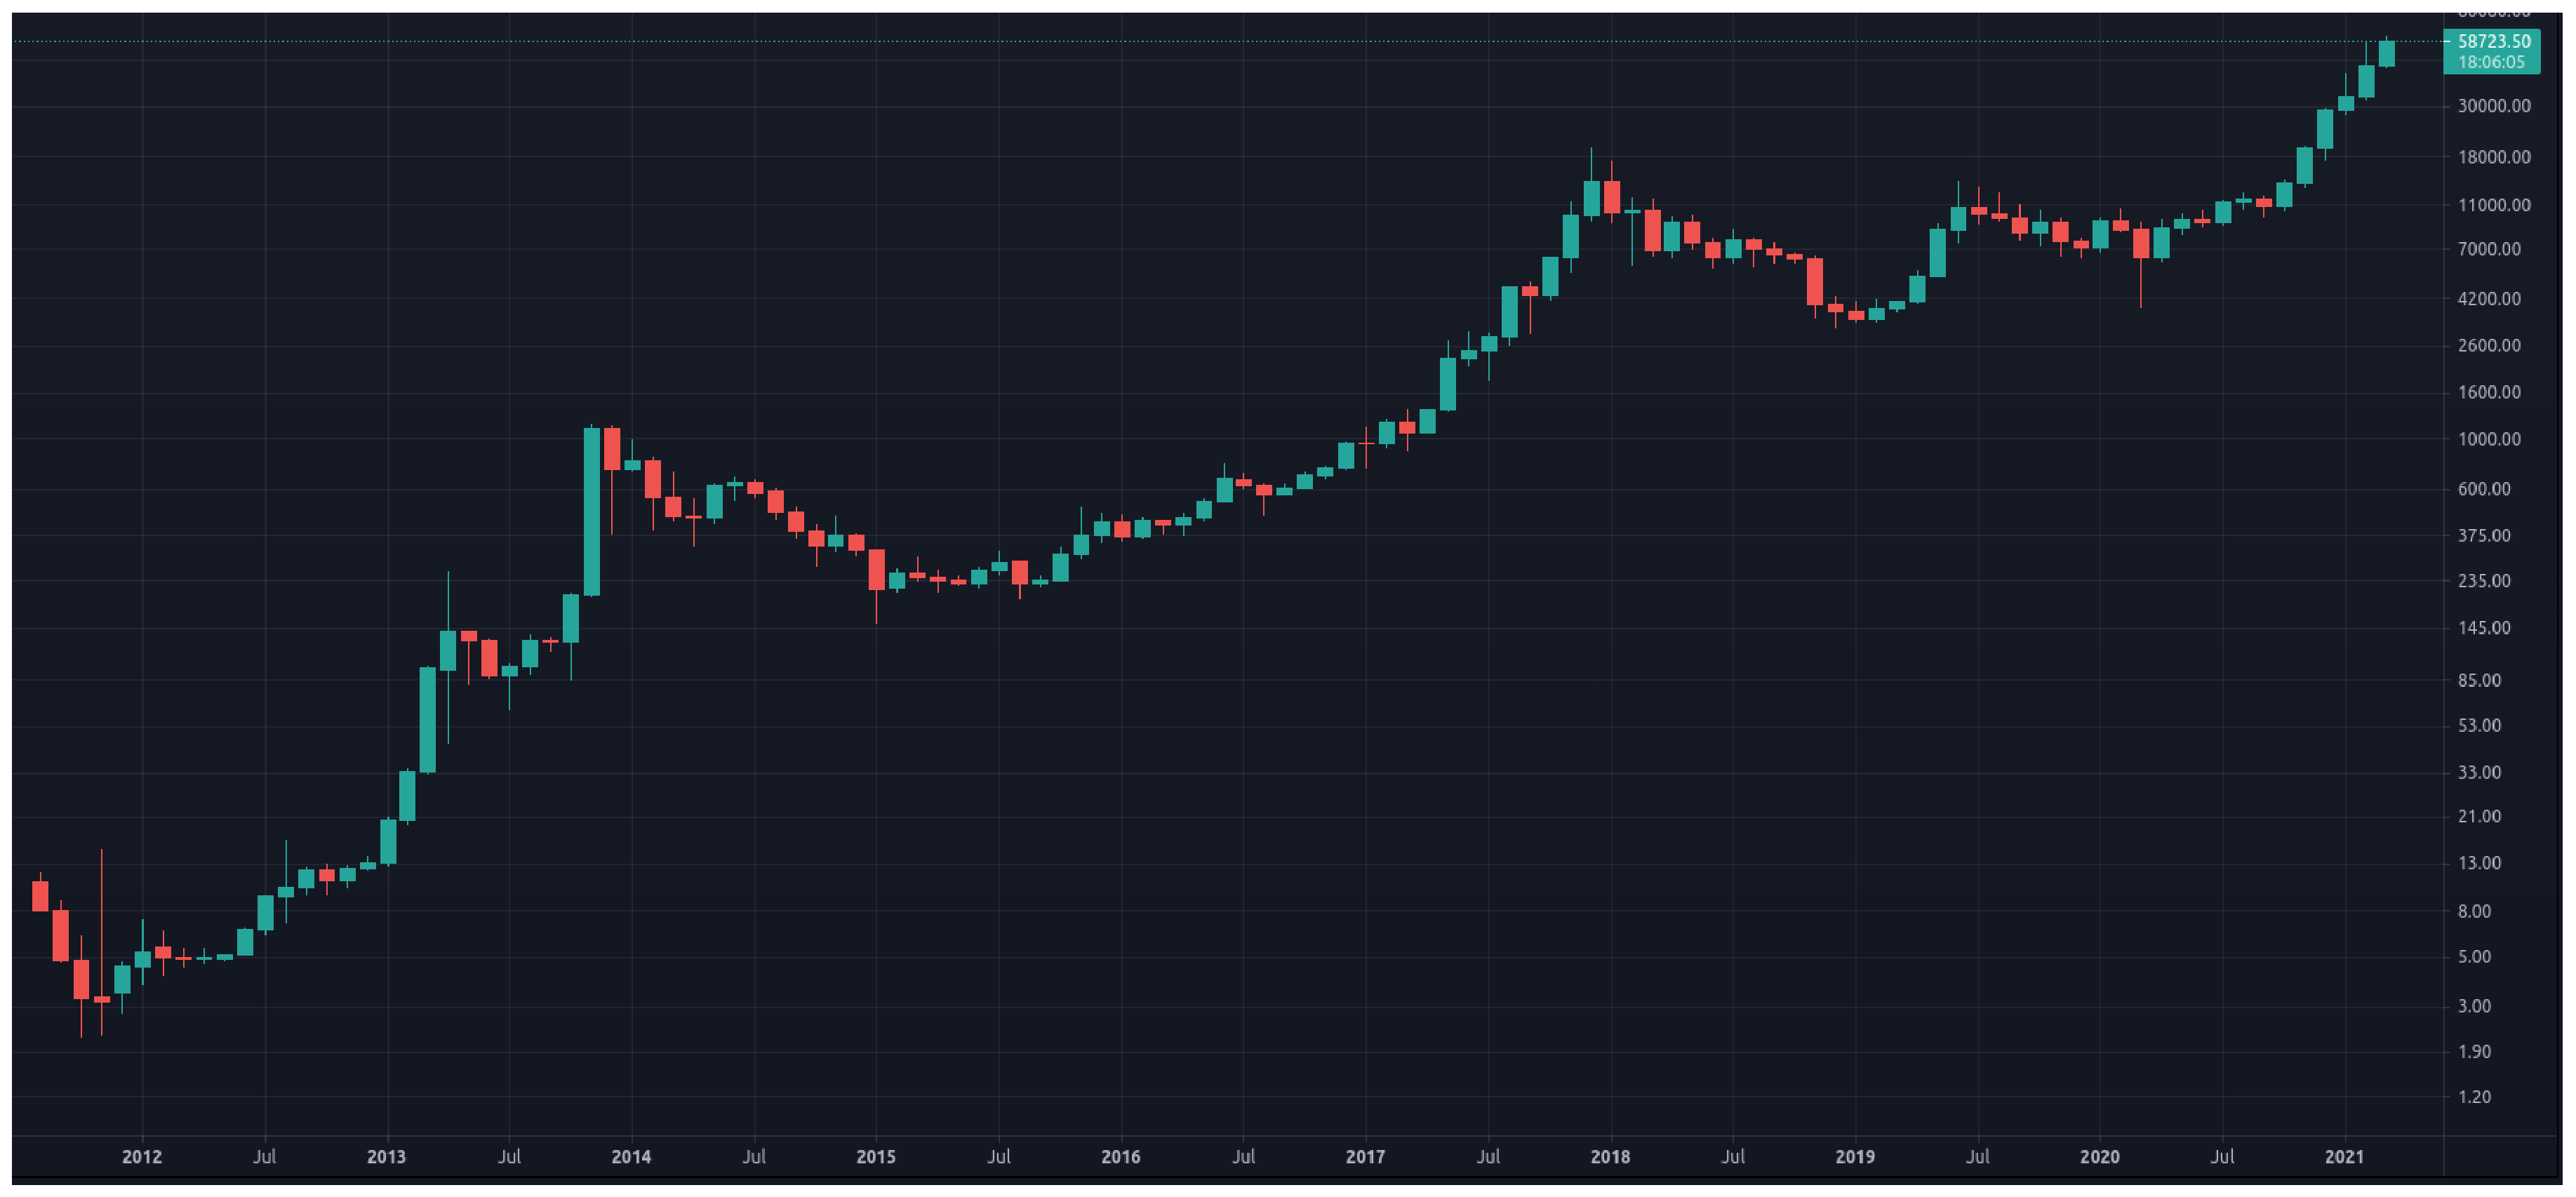
\includegraphics[width=\textwidth]{figs/btusd.eps}
% \caption{BTC/USD}
% \label{fig:btcusd}
%\end{figure}
\begin{figure}
    \centering
    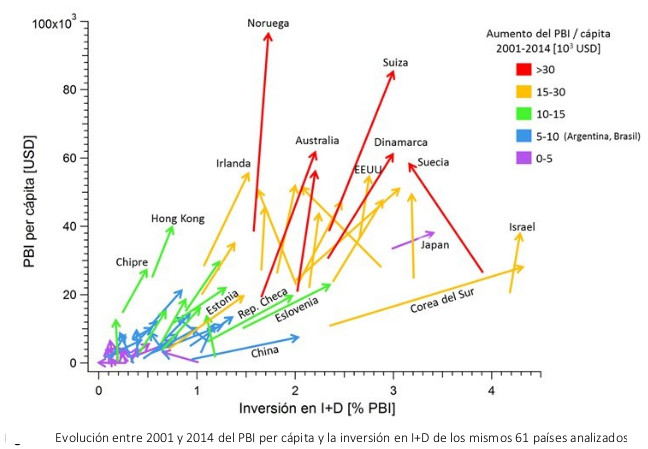
\includegraphics[width=0.5\textwidth]{figs/Docuemnto_Stefani_2.jpg}
    \caption{\href{https://aargentinapciencias.org/wp-content/uploads/2019/05/Docuemnto_Stefani.pdf}{Congressional Report, Prof Stefani}}
\end{figure}
\subsection{Indexing Open Production and Development}

If Bitcoin/Blockchain is a decentralized technology, its use as a store-of-value for Astronomy must complement decentralized education, research, and development. This is embodied in its name-sake, so-called term: "Open Development".

A community defined and validated AOD system could be used to evaluate preferred funding channels including node validation via incentives Txn types. Such a system could be periodically revised by the community with community governance protocols that ideally would respect yet complement existing structures in a self-consistent decentralized manner. IVOA could be the perfect example with 19 Nation State member countries and 4 international members. These metrics could be used to direct and supply liquidity for the Open Development of Astronomy. As seen in Fig Seffanni. national governments that spend a larger percentage of GDP towards science and technology also on average have higher GDP growth rates (in USD). So this could be a weighting factor metric. See equtation1. Reciprocal percentage of total GDP towards science could be a constructed normalization parameter. So too could total debt to GDP public debt.  An example is the Maker ERC231 ETH governance token that itself control a  pseudo-decentralized US stable coin bank, DAI, over-collateralised that has remained 1 USD for several years despite the BTC market varience.  On the question of whether a special token need minting. The pros and cons need to be carefully studied by the community. For example WETH and WBTC are stable tokens that are on native ETH but allow interconectivity between chains. A similar system occurs with the price issuance of DAI via Maker. It is an important element of DEFI and governence that is included in Figure 2.   

DEFI protocols and more general community may have some motivation to provide decentralized funding for astronomy Open Development. First, Open development protocols could insure existing methods and procedures may also be applicable to the Open Development of Astronomy Community. Both  based on Open Source technology, that follow the Lindy effect.

 \begin{figure}
    \centering
    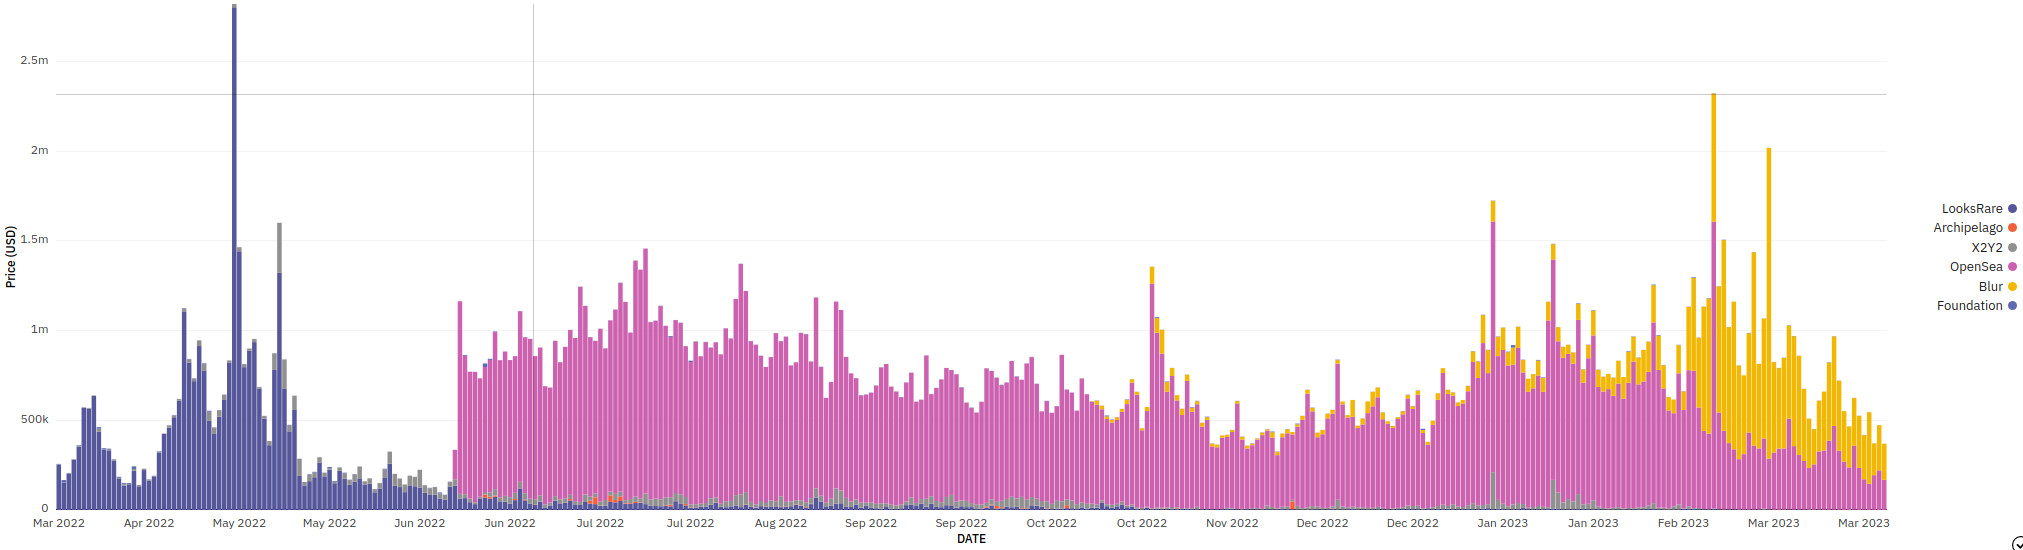
\includegraphics[width=0.5\textwidth]{figs/royalty_pay.jpg}
    \caption{Ethereum Token NFT royalty payments}
\end{figure}
\subsection{Model Attributes of a Token for Astronomy}
\label{subsec:btc4}
There are certainly advantages if the community has its own token. But there are also disadvantages. RSA Ecliptic Curve Algorithm, asymetric hash function, Blind, Schnor Signatures, Merkle Trees, ZKP,  WEB3, Multi-sig, Cross chain, mixing - Privacy. 

\subsection{Block Validation}
\label{subsec: validator}
Blockchain Validators and Nodes. ERC20 Protocalls like GRT ERC   

\href{https://defipulse.com/}{DEFI$\;$ PULSE} pulse is a list of all the liquidity that is tied into DEFI. There is over 77.77 $\times 10^{9}$ USD locked in DEFI. The UNISWAP treasury has in excess of 3 billion dollars. These treasury funds are available via grants programs that Astronomy Open Development protocols should have access to.

In this section, a toy model for the open development of Astronomy based on open Blockchain technology is presented. An attempt is made to sketch out ingredients and methods of a `successful' model. Some elemental principals as voted by governance should be voted at different stages calibration proposals. For argument sakes in this model we follow the UNISWAP snapshot community, where there are different instances of governance. We also have a treasury funds, and the like.  through governance solutions. The UNISWAP model, to date is one of the largest decentralized exchange, has many developers working for it, was the first massive airdrop token of Blockchain value, so is essentially decentralized in our assumption. The funds for this Paper come from DEFI, from the NOVA node of the IVOA-EXEC committee for Argentina. Some fundamental actors are identified and their functionality with the model sketched out. This paper does not pretend to discuss in strict technical details the finer points of the implementation of such model and parameters therein, but does make reference to some basic cryptographic primatives including Merkle Trees, Zero-knowledge proofs, cross chain protocals, etc. that offer promising solutions and could certainly be considered to be incorporated during Improvement Proposals directed by the community periodically. The paper does not delve into technical details of some Blockchain procedures like mixing to maintain secure personal and private information but of all actors but pretends to highlight some core model features to be followed up by future authors but obviously  locked value will naturally flow to the more useful protocols.  
 
The only condition to participate is bonafide scientific curiosity for Astronomy so sufficient incentive methods need to be developed to entice value-added interaction with the astronomy Blockchain via Decentralized Block Chain Applications, (DAps) as programmable parameters that can be set by the Model's governance component albeit individual minority actors. 

%This part examines a type of Model. The ICO era based on the Ethereum smart contracts bubble that burst aside from rthe egulatory issues about Securities that was mostly based on near useless speculative tokens must be avoided by any AOD bonafide . It looks at some main or speculive  I would not be in favour of an ICO, I think founds are complimentary and as such must come forom existing DEFI protocol pools. But the Community must decide this. However, For the sake of simplicity the following three `actors' are identified as founding governance members: International Virtual Observatory Alliance, the  Astropy community and authors of referred peer reviewed journals weighted by their h-index, the International Astronomy Union etc. Parameters such as the weight of each should be set soon and be discussed by the community and there could even be a switch or that must be voted on according to community established acoords. For example astropy community. A type of switch could be voted for to change the relative percentage of votes.UNISWAP for exmaple is the first governence token that inclduded the AMM liquidity  The reward will be the AstroOD Token, since the wallet creation, Blockchain exploder and DApp python tools and protocols are unified by the proposed affiliated package of astropy. This parameter could be considered to as a proportionality of any initial coin distribution function. But we would be against this and think programs need to start from the ground-roots up, providing liquidity and rewarding Tx were useful (community validaded) Tx occur. On Balance an initial token distribution or ICO has drawbacks and so our model draws on existing liquidity pools from the DEFI Space.

Over 70 percent of Astronomers use  Astropy and recent paper in preparation show a promising metric in developer community as the community developer toolkit for Open Source code, that with VO software makes up the majority toolkit of astronomers barring some HPC computing for N-body simulations. Many astronomers probably agree to say these would be the recognized go-to  Astronomy Software and Development so the Astropy Community onboarding, usefulness would be advantages to the Open Development Astronomy model (here-after ODM) of Astronomy as proposed. Affiliated package authors could be validated and offered a period to open a wallet and partake in governence DAO. An affiliated package to Astropy is selected to generate private public SHA256 pairs and the generated funds will be locked by the Community 70 percent to Developers. 

No initial coin offering is neesary as this would be deemed a securtiy and may violate some Legal Juristicitions that we argue for Open Development must be lawful yet, at the same time decentralized means if a majority want and if safeguards are put in place, ie truelly decnentralized nodes, not INFURA WEB three but above. So recognizing `challanges' that Open Protocol must face and converging on Wrights Law of the CDF of Astronomy Developement we appeal to DEFI grant protocols to fund our development. 


The AstroOD package 

We propose an AstroOD coordinated package \textcolor{red} github ref. that periodically receives data-feeds on AstroOD on collects basic statistics of packages being used and is correlated to ADS Main-Text query and ORCID query. A possibility is to build a SubGraph to program as an Oracle on UNISWAP. UNISWAP liquidity    Anyone in the Astropy community can create key pairs to be used as Smart Contract accounts. The program using RSA, and blind signature for privacy. The package will include a functional wallet, with multi signature, multi currency and multiple accounts. This will be the basis of deployment of “Smart Contracts”, as a concept was introduced in 1995 by Nick Szabo, who described Smart Contracts as “a set of promises,
specified in digital form, including protocols within which these parties perform.

AstroOD package will have to be built to implement the use of Oracles, to connect the community to the Blockchain space. Oracles manage feeds of information are not put into the native Blockchain due to scalability or privacy issues, etc but to other Chains.  Oracles are more focused on price-feed data for crypto asset prediction markets but with DEFI burgeoning and necessity the Oracle inputs are becoming more diversified.  The Oracle Problem 4 promises” (Szabo, 1996). 

Feeds for Oracles would include ADS-NASA, ArchieX ., etc,  to validate information that can be used to automatically set parameters in the model. The weights could be voted on by IVOA representatives.

If the  model truly represents an open Blockchain then anyone can participate and be offered rewards as incentive in pursuit of open astronomy. It is obviously important that protocol standards be defined and a body like IVOA could be instrumental in helping to define them with the Astropy community, for example. That body could take into account validaded economic considerations like inflation of national currencies., crisis, etc. Staked AstroOD tokens can be awarded using a 'competative' awards scheme program to Secondary School Teachers, Plenetarium guides, thesis graduate students etc. that work to teach astronomy. All must have oportunity to receive incentive rewards for their valid contributions including for example validated University students and volunteers that mount Open-Day/Night activity for the public, etc., All should receive incentive rewards for their contribution since sacrificing their time in sharing knowledge to allow others opportunities should be rewarded as it is clearly in pursuit of Open Development. Weightings for these activities can be set periodically by the governance component with mandatory revision periods, and clauses if they change too abruptly. An option is to follow MakerDAO governance models, with funds from Treasury. Unfortunately political, financial, health  crisis cause by rampant financial speculation and the like, will probably not be solved by Central Bank Digital Currencies, as these are essentially still centralised institutions on a Blockchain.  Often during these crisis outreach and educational activities are the first casualty of open development, as are essential and scares resources for Public University and National Institute research bodies. In the case of the creation of events, the governance model will award staked token holder to provide credit for future open development. Authors who publish papers also may claim awarded tokens and trade them too?

\subsection{Digital Open Ledger Technology}

\subsection{ERC 721 }

ERC 721 tokens are an ETH standard token contracts that are Non-Fungible Token (NFT), ie they are unique and indivisible or in other words can be used to identify a unique event, object or condition. This type of Token may be used on platforms that offer digital collectibles, access keys, lottery tickets, numbered seats for concerts, sports matches or academic meetings, for example best "student" poster prizes in conferences, etc. 

ERC 721 tokens may have different values from one another although derived from the same Smart Contract base, due to its age, rarity often iconized by its unique visual artistry (appearance).

The uint256 variable or called tokenId, so for any ERC-721 Contract, the pair contract address, uint256 tokenId must be globally unique. Said that a dApp can have a "converter" that uses the tokenId as input and outputs an image of something cool, like zombies, weapons, skills or amazing kitties!


With PAOP protocol ERC721 SMart Contract Non-Fungable Tokens can be issued on demand if needbe. These digital collectables will be sold on a Dex funded exchange, to provide liquidity to further Scientific-Cultural use-case.

i) A PhD scholarship holder has run out of PhD Funding 
ii) A Group that is working in some country has had the USD devalued and the subsidy payments are late, and they are applying for some tokens and offer in exchange a collaborate NFT to be published in the acknolodgements of the paper.
iii) A group of astronomers, technicians, students,  are building an observatory in a advantageous site in a poor country. 

\subsection{Tokenisation}

Since centralized regulation that at some stage may undermine public open Blockchain science development and by weighing-up pros/cons between POW and POS consusus, of the Table blockpros/cons as well as from recognizing the 12 year dominance of BITCOIN we choose to follow governance model tokenisation, adopted by  companies like "Shape-Shift" a XXX billion USD companies that has become completely Tokenized. Any system must be able tp use Bridges even to different chains. 

Its xxx workers were each given some tokens as where select members from the community. 

A possible route of course is to solicit an initial token grant from UNI the largest decentralized exchange provider as well as other DEFI DAOs, then in an active campaign period leading up to the token release allow for initial KYC. Since We need to validate some key actors that include students that are doing a graduate or undergraduate degree with major in Astronomy professors of Astronomy Univsersity Courses. Developers, authors and co-authors of open development astronomical software, including those of affiliated packages in Astropy. 

\subsection{Initial Token Distribution}
%This part so far just fun ideas but not so in favour of having an ILO or ICO etc., thinking the CONS are to stacked up against it but eventually Authors and co-authors Via the MNRAS sites and some form of Zero Knowledge Proof Validation will be able for each paper publishes list astroOD, that will be obtained from Treasury.

\subsection{Liquidity pools}

Liquidity pools for Astronomers , Travel Conferences, Observing, Teaching, these pools can be flexible but it is advised to be a percentage of PhD  students or some metric related to PhDs produced. 

\subsection{Career Development in Astronomy}

Over the time-scale of 3-5 years, incidentally about the time it takes a new astronomy major to complete a PhD, Bitcoin and perhaps some other OB like Ethereum have stood-up to their promise hold store of value properties. Bitcoin was born after the 2008 sub-prime morgage backed security and credit default swap crisis when the worlds largest banks and insurers were called to account since they were instrumental in the greatest financial crisis since the great depression of 1930's and had to be bailed out to prevent global contagion effect.
 
For the astronomical community in Argentina a similar debt crisis has put the Argentina Gemini membership under threat since in 2020 a consortium decided on behalf of Argentina to offer partial withdraw. A situation that unfolded since only a small fraction of the funds required by the Gemini consortia on behalf of Argentina for 2019 were paid by the previous government and similarly astronomers wages and subsidies perceived to be undervalued. Unfortunately the news for science in general was not great since the Ministry of Science was disbanded and funding to host international conferences in 2019 were unavailable. Although the new government did fund a new Ministry for Science, and Blockchain technology is considered a strategic area, there is not much OB development from CONICET. If adequate funding is not forthcoming these types of crisis like is likely to be the case for other countries with large USD dinominated debts cause more difficulty in the educational scientific and technological ecosystems that may include new brain drain waves for young-scientists leading to a spill-over exacerbated and undesirable effect as talent settles overseas. 

This dire context above was contracted in complicity with loan requirements, exerted by the International Monetary Fund through loan obligations and/or conditioning that prioritized a creditor bonanza scheme based on a 70\% bank lending rate set by the PRO party coalition led by the ex-president of Paradise Paper's acclaim that ran a coalition government to full-term. 

Underlying this debt ridden situation, is a loaming world recession within a COVID-19 pandemic context with the cancellation of international Astronomical conferences, workshops and other meetings is taking place at a global scale: IVOA was forced to change the meeting mode and since the May Sydney Interop until 2023 all meetings have been virtual, and  in Argentina the Observatory Astronomical of Cordoba (circa 1873) one of the first national scientific institutions with the Instituto de Astronomia Teorica y Experimental announced the suspension of the 2021 Friends of Friends workshop. 

It is argued that the current crisis, like the last major one that affected the research capacity of scientisits to conduct their work in Argentina was the 2001 economic crisis, when Argentina paid for being the "poster child of the IMF" with the greatest default in history and before that, when the Argentina Scientific output capacity was being determined down the barrel of a gun by the military junta and some home-grown scientists that would probably prefer to stay unnamed that seemingly justified this collateral damage (see Nature Levato paper, that was arrested in what appears a Mysogenic probably unrelated case.

In this context and given the fact that the half-life rate of Astronomy majors from US public universities has been in steep free-fall.  \cite{milo_2018} it is that the discussion of incentivizing using Blockchain tokenomics. At the same time, government spending in the military industrial complex, banks, insurer and corporate bail-outs are at an all time high so as scientist it could be argued that it is our responsibility to add checks and balances with recognizably proven community technology. 
%
If such a model exists it is certain that data Feeds protocols will become an important part to allow to mitigate mistakes from central actors since the system must be largely transparent yet private when it needs to be. Our model would use Zero Knowledge Proofs and other Blockchain primitives to safe-guard privacy of information of the individual yet also compensate or incentives the brave. 
   
The identification of elements or properties for the programmatic `tokenization' of an open development protocols for astronomy should not be influenced by any one central authority nor by extraneous factors affecting the wider political economy but should be decided by the community and based heavily on open source and open development paradigm. 
   
In section \ref{sec:intro} we stated the motive and underlying potential of applying open development technology to astronomy. We detail with warp speed some crytographic primitives (Has functions, Merkle roots) and some basic protocols to establish a general model frame-work of Tokenomics, including staking or yield-farming incentive mechanics, time and value locked development fund release functions, and also discuss the implications of governance, etc,

\section{Onboarding}
\label{sec:use-case}

IVOA partners could run full nodes, to validate the Bitcoin blockchain.

A full node could be run for less than 300 USD a year. The advantages of running a full node are:

1) Tap into trustless lightning network in a non-custodial way. This is to store non-custodial payment channels on layer two of the Bitcoin network which would provide privacy 

2) Obtain validation fees for node members by processing transactions


Liquidity is a necessary resource of any token model. Our Open Development Model requires liquidity. The patch offered here is to tie into the liquidity pools of the decentralized finance movement that we would hope to form a common token fund. Some parameters of the funding rate, principally by UNISWAP grant, would be determined by that community.   

\section{Case-Study}
\label{sec:btc5}

\begin{itemize}
    \item{SSO SSS defence contractor that had previously developed ordnance systems on weapons that served in the Illegal war in Iraq was knowingly selected to build the Sky-Mapper detector. } 
    \item{NSF Shutdown or Telescopes in EEUU during Obama and Trump administrations}
    \item{Split decision of the Australian community under the Hawke government to direct funds to upgrade of radio-facilities in Australia, instead of ESO membership}
    \item{Close door period of Scientific Research position in Argentina, 1990's}
    \item{Gemini contractual issue for Argentina, implicating a withdraw of funding from the ministry of funding, and a divided community because of recommended reduction of Gemini time.}
    \item{NFT for the MOA}, see Figure 1, which the Astronomical Observatory of Cordoba holds NFT ownership and wishes to sell for to help fund the MOA and research activities. 

\end{itemize}


\section{Decentralized Finance} 

Case study of NFT
\begin{figure}[ht!]
    \centering
    \label{fig:my_label}
  \caption{NFT collectable, world event to constrain Einstein's GTR before publication, foto by the C\'ordoba Observatory team,
during the 1912 eclipse expedition. The Perrine settlement is located in the right, attached to the big white building. Courtesy of the Museo Astron\'omico del Observatorio Astron\'omico de C\'ordoba, C\'ordoba, Argentina.}
  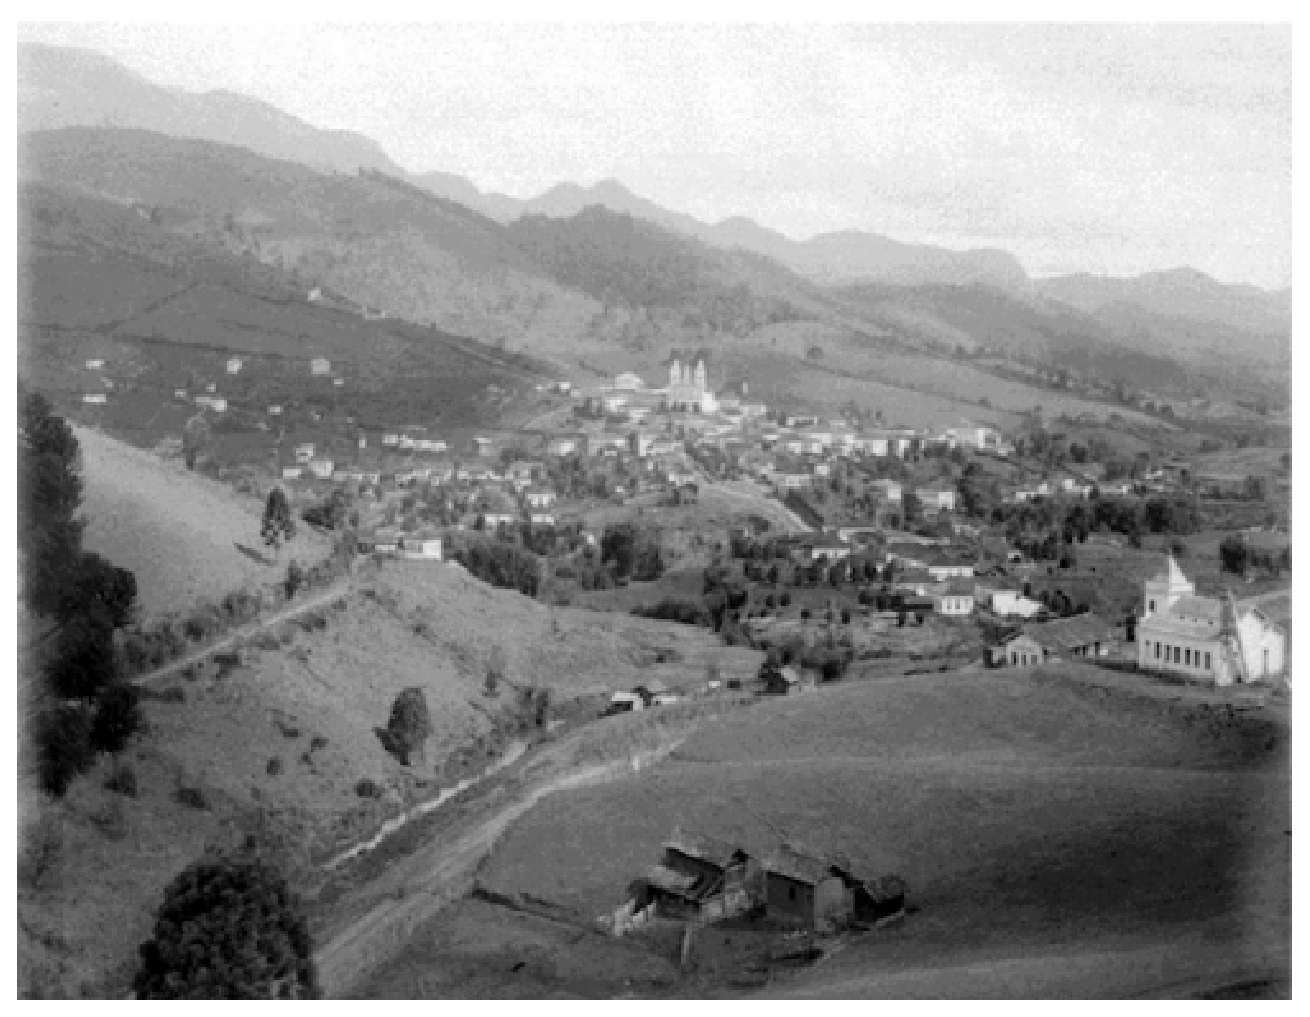
\includegraphics[width=0.4\textwidth]{figs/p1912.eps}
\end{figure}



% =============================================================================
% Smart Contracts
% =============================================================================
\section{Context}
\label{section:context}
%


% =============================================================================
% POAP.xyz
% =============================================================================
\section{Developer tools}
\label{section:Eth721}
%
We consider that since astropy is the leading open developer toolkit for astronomical research reflected in the astropy  user and dev comits see \cite{ 2020ASPC..522..491T}, that it be used at t0 launchdate but details could even be revised later by governance.  The Etherium Blockchain contains a type of smart contracts called NFT or non-fungable token.  This type of token is non-interchangable can be unique to preserve the notion of digital scarcity, and can be verified without any centralized organization required to authenticate it. These smart contracts can be used issue incentive rewards to nodes. A protocol build around 721 protocal includes POAP.xyz, ref(github address). This proof of attendance protcol can be used to validad the attendance of astronomical events, including virtual ones. The tokens can be exchanged for goods and services and soldon for fiat money.  


Data feeds will be entered into Oracles that will automatically via smart contracts provide incentive rewards to the node and user wallets.
%
POAP type proof of attendance protocol for meetings. To rewards students for attending and presenting their results in meetings.
%
\subsection{Hash Function Account}
We propose for any developer of Astropy core plus afiliated package models including co-authors are onboarded and in our model we apply the afilated package astropy Package astrobtc, recognizing the fact that Bitcoin has been the major asset class for the last 12 years that included several global crisis. 
%

Astropy proving to revolutionize astronomical data-reduction collaboration and is channelled through the open development of astronomy project Astropy. It involves IVOA's 20 member institution was originally much smaller and conceived by its founding members to be a large fraternal virtual observatory working seamlessly in perfect collaboration with no imposed boundaries other than those of the ethical nature. Today it consists of mostly national VO members as well as three very important international members that include: the European Space Agency, the European VO and the UK VO. The national members are: Argentina, Armenia, Australia, Brazil, Canada, China, \textit{Europe}, France, Germany, Hungary, India, Italy, Japan, Korea, Russia, Spain, Ukraine, the United Kingdom and the United States. This `paper' proposes to open the discussion on the adoption of Block-chain technology for IVOA for the open development of astronomy. It is written in the context of long term flaws experienced in the current development model paradigm that results in less than efficient research inventive mechanism and cyclic funding crisis as well as possibly serendipitous COVID-19 type pandemic that may become more frequent.
%
Aside from some issues as illustrated below that would pausibly affects any 'closed' development model for astronomy, or one determined by powerful central actors, one based on open Blockchain technology should, on the other hand preferable gravitate to real open development via carefully thought-out and implemented incentive mechanisms to foster collaboration in a more efficient way and lay the path to unprecedented scientific discovery and innovation. It is in this context that I invite the reader to contemplate on the opening discussion of IVOA in the field of tokenomics. 
%
Our analysis focuses on the US public university research system, some limited experience on the IVOA system and the Argentine, Australian astronomical research system. 
   
   Strong motivation for this discussion is based on the facts that:
   
\begin{itemize}
       \item A dwindling half-life for the Astronomy and astrophysics PhD majors in US, Australian \& British (etc,) public university system meaning astronomy and astrophysics is loosing a main investment, its researchers.  
       
       \item Shortfalls caused by ciclic funding crisis that affect education institutions, scientific research facilities observed as acute funding restrictions, cutbacks and "government shutdowns" and/or inflation in national currencies, is the elephant in the room that must be addressed.
\end{itemize}
       
       
This paper argues the use of "Blockchain Technology" as a necessary tool for efficient and sustainable open development in Astronomy as an underlying incentive mechanism for collaborative research projects that foster open development community identified metrics.  


% =============================================================================
% SECTION CONCLUSIONS
% =============================================================================
\section{Application prospects}
\label{sec:5}
%
In this section we look at possible paths to embrace AOD onboarding. To secure the network we recommend all existing IVOA members run a full Bitcoin node. A full node can be run on a Raspberry PI.  This will allow all node operators fast lightning censorship free payment channels. Recomendation is that this node be set up as a multi-sig scheme. Also proposed is an affiliated package to Astropy AstroOD to build on the DEFI stack including the creation of wallets and metric based discussion group for open software development in consultation with the Astropy Finance Committee. This new package developed by the community must be compatible with up-coming Python versions and be fully documented in a public repository. Another recommendation for is a multisig signature WEB3 wallets operated by all IVOA representatives in association with the project observatory chair, vice-chair and representative . A 2-3 or 3-5 multi-sig scheme would suffice. Finally an IVOA/Astropy Uniswap governance proposal for the seed-funding. This proposal must go through 
 Phase 1: Request for Comment (RFC), Phase 2: temperature check and finally Phase 3: Governance Proposal, see Fig \ref{fig:unigov}
%
\begin{figure}
    \centering
    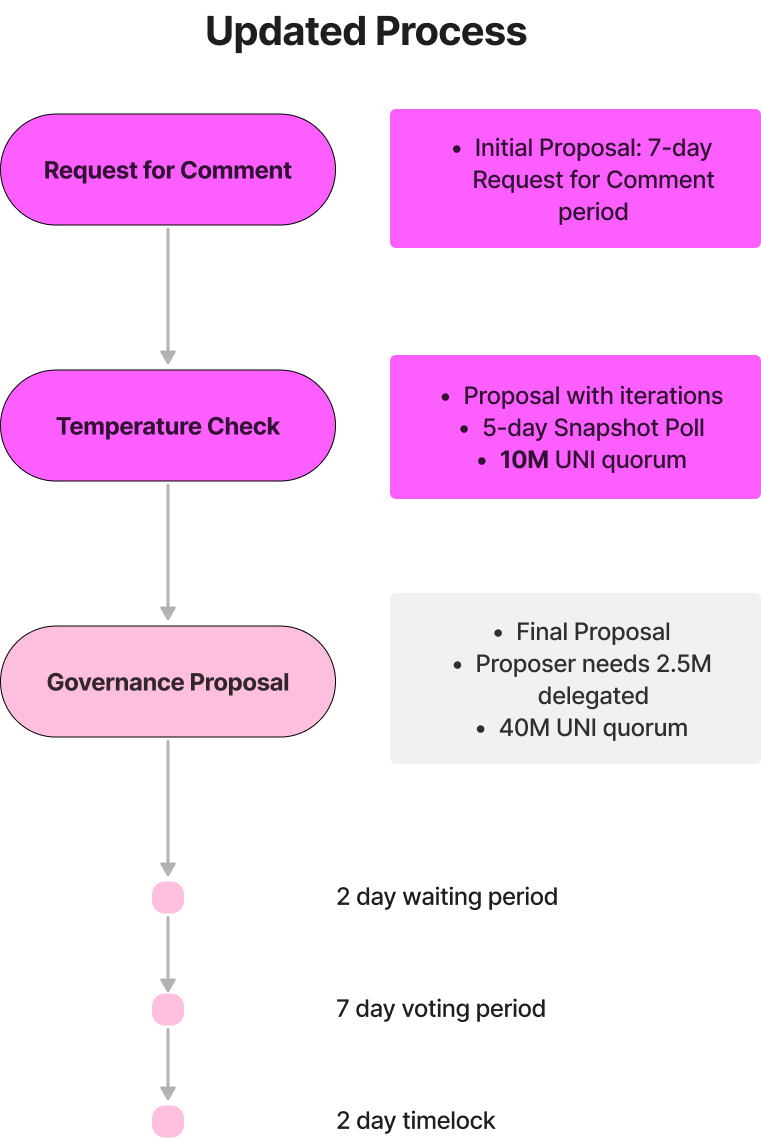
\includegraphics[width=0.38\textwidth]{figs/unigov.png}
    \vspace*{-0.2cm}
    \caption{Uniswap governance proposal}
    \label{fig:unigov}
\end{figure}

Future development will focus on the following three areas: incorporating
new features, improving documentation, and 
possible integration with tools for interactively analyzing features of development.

IAU and IVOA Astronomer data-base to validate KYC, coordinating contact with different institutions. 

% =============================================================================
% SECTION Acknowledgments
% =============================================================================
\section{Acknowledgments}
SG acknowledges the New Virtual Observatory of Argentina (NOVA) and his selection as representative of Argentina on the IVOA-exec committee and support of all his colleagues in the IATE.

% =============================================================================
% SECTION BIBLIO
% =============================================================================
%
%\section*{References}
%\label{biblio}
\bibliographystyle{model2-names-astronomy}
\bibliography{ivoatoken}


\end{document}

\endinput